\documentclass[a4paper, twoside, 11pt]{report}
%pridat documentclass[twoside] - pro tisk
%\input{thesis_settings/page_settings}
\usepackage{xcolor}
\usepackage[colorinlistoftodos, textsize=tiny]{todonotes}
\usepackage[top=2cm,bottom=2cm, left=3cm, right=2cm]{geometry}
\usepackage{graphicx}
\usepackage{wrapfig}
\usepackage[utf8]{inputenc}
\usepackage[linktoc=all]{hyperref}
%\usepackage[czech]{babel}
\usepackage[utf8]{inputenc}
\usepackage[T1]{fontenc}
\usepackage{needspace}
%\usepackage{fontspec}
\usepackage{calc}
\graphicspath{ {images/} }
%
\newcommand\pro{\item[$+$]}
\newcommand\con{\item[$-$]}
%

\usepackage{calc}

\begin{document}
%
\begin{titlepage}
\title{Introduction to\\Additive Manufacturing Technologies}
\author{Martin Hejtmanek}
\date{28.2.2017}
\maketitle
\end{titlepage}
%
%
%
Tato stranka bude nahrazena zadanim prace
%
%
%
\newpage
\vspace*{\fill}
\LARGE
\noindent
\textbf{Declaration}\\[10pt]
\normalsize
I declare that this bachelor project is all my own work and I have cited all sources I have used in the bibliography.
\\[10pt]

\begin{figure}[b!]
\begin{minipage}[t]{0.3\textwidth}
    Date
    \dotfill
\end{minipage}
\hfill
\begin{minipage}[t]{0.3\textwidth}
	Signature
	\dotfill
\end{minipage}
\end{figure}
%
%
%
\newpage
\vspace*{\fill}
\LARGE
\noindent
\textbf{Acknowledgement}\\[10pt]
\normalsize

	First and foremost, I have to thank my thesis supervisors, Mr. Jiří Moravec. Without his assistance and willingness to help me throughout the research, this thesis would have never been accomplished.
	

	I would like to show my gratitude to Mr. Esa Kontio from Oulu University of Applied Sciences, for introducing me into the field of additive manufacturing. Only thanks to his attitude during attended lectures and willingness to dedicate his free time to help me with school project, I developed enthusiasm for additive manufacturing and chose to pursue it as the topic of my bachelor thesis.
	
	
	I must also thank Mr. Josef Průša, for his goodwill to cooperate with me, and providing me with necessary equipment for the practical part of my thesis.


	My sincere also belongs to Ms. Zdeňka Jeníkova from CTU's department of material engineering, for her time and possibility to use local amenities, that allowed for the practical part of the thesis to take place.
	
	
	Finally, I can't but express my deepest gratitude to my family for the support during the time this thesis was being created.
%
%
%
\newpage
\LARGE
\noindent
\textbf{Abstrakt}
\normalsize
\\[10pt]
Tato bakalářská práce se zabývá aditivními technologiemi výroby. Je zde popsána souvislost mezi aditivními technologiemi a procesním inženýrstvím. Následující popis a souhrn vlastností jednotlivých technologií slouží pro vytvoření základního uceleného obrazu a jejich možnostech použití. Závěr práce se věnuje výzkumu pevnosti tištěných vzorků v závislosti na výrobních parametrech.
\\[20pt]

\Large
\noindent
\textbf{Klíčová slova}
\normalsize
\\[10pt]
Aditivní technologie, 3D tisk

\vfill
\LARGE
\noindent
\textbf{Abstract}
\normalsize
\\[10pt]
This bachelor's thesis is focusing on different additive manufacturing technologies. There is description of the relation between the additive manufacturing and process engineering. Following description of various additive manufacturing technologies should serve as an introductory educational material. The last section of the thesis focuses on the effect of printing parameters of FDM technology on final part's strength.
\\[20pt]

\Large
\noindent
\textbf{Keywords}
\normalsize
\\[10pt]
Additive manufacturing, 3D printing, stereolitography, powder bed fusion, material extrusion, material jetting, binder jetting, sheet lamination, directed energy deposition, tensile strength

\tableofcontents

\chapter*{List of shortcuts}
\addcontentsline{toc}{chapter}{List of shortcuts}
\begin{itemize}
\item[AM]Additive manufacturing
\item[BJ]Binder jetting
\item[CNC]Computer numeric controll
\item[DED]Directed energy deposition
\item[DMD]Digital micromirror device
\item[DMLS]Direct metal laser sintering
\item[EBM]Electron beam melting
\item[FDM]Fused deposition modeling
\item[FFF]Fused filament fabrication
\item[LOM]Laminated object manufacturing
\item[MJ]Material jetting
\item[PBF]Powder bed fusion
\item[SL]Sheet lamination
\item[SLA]Stereolitography
\item[SLS]Selective laser sintering
\item[STL]Stereolitography or STL file format
\item[UW]Ultrasonic welding
\end{itemize}


\chapter{Introduction}
%
%
%
\section{What additive manufacturing}
There are many terms like Additive Manufacturing, 3D printing, rapid prototyping and more, that are used to describe specific technologies. Although they are not precisely synonyms, all of them are related to a specific way of product manufacturing. Nowadays, we are still used to make machines and parts from solid blocks of raw material, and then machining away material until desired shape if acquired. Also casting, forming, welding and other technologies are used in the classical process chain, in order to make a specific part.\\
However, since 1980s there were new and different manufacturing technologies being developed, that used vastly different approach. This trend still continues with more and more interest being paid to this field. Those technologies are commonly named Additive manufacturing technologies (hereinafter AM). The main underlying principle of all AM technologies, that will be listed later, is making part by adding material, instead of removing it. This approach has many advantages over previously mentioned conventional technologies, but it also brings different problem sets that need to be solved.

	As mentioned, AM technologies are on a rise. It is now more than 30 years since humble beginnings of the first AM technology, Stereolitography. Since then, AM industry developed rapidly and is today worth several billions of dollars on the market. Its significance can't be stressed out enough, and sometimes we are not paying as much attention to AM as we should. It takes a lot of time to fully realize, how big difference in terms of parts production AM can cause. Sometimes we might not realize, that parts we are used to make using classical approach, could be made using AM, faster and without perfectly planned pre-production planning, post-production and with less waste material. AM technologies were not developed to replace conventional technologies - they will probably always have its place on the market. Still, conventional processes can be supported by AM when possible in order to increase manufacturing speed, simplicity and reduce product price. There are even available machines, trying to merge CNCs and AM into a single functional production machine.
	
	The future of AM market is still to unfold, but statistics are showing that AM machines will be used more in production process - especially with the continuous trend of improving materials availability, development of new materials or price reduction of all key electronic and mechanical parts. With this trend, demand for AM AM specialists is likely to increase.
	
\section{Goals of bachelor thesis}	
	The main goal of bachelor thesis (BT) is to make research on the AM field and available technologies. Then, make a brief, but complete and understandable summary of them and describe ongoing processes. This BT should give the reader an opportunity to understand essentials of individual technologies - know their strengths, weaknesses, main working principles and for which applications are they suitable.
	
	For the problematic of AM machines is very complex, choosing a single technology and fully describing it into detail would be sufficient for diploma thesis. Therefore it is out of scope of this BT, to give detailed description of all technologies. There are many intricate processes included, related to heat and mass transfer, material processing and properties, precise positioning systems, careful regulation of build environment conditions and much more.
	\newpage
%
\section{Resources}
In this thesis, I use primarily limited amount of resources and literature. Even though this thesis should be complex and diverse, I decided to use the book \cite{AMT} as my primary source of information. This book is than supplemented by facts from scientific journals, other books, information from AM machine vendors, webpages and others. Also, there are sections where I write information gained at OAMK - Oulu University of Applied Sciences (mentioned in the acknowledgement).

	The reason for using \cite{AMT} as my primary information source is following - this book is up-to date (2nd edition, 2015) and goes deep into the topics well enough, citing on it's 500 pages more than 200 journals, publications and other information sources. It also includes both theory and practical examples from industry, covers all the details of almost any AM-related problematic and full understanding of the whole content requires high level of education in chemistry, calculus, material engineering and more. Since it is at this moment out of my scope, even to fully understand this book itself, I believe taking it as a primary information source is acceptable.
%
\section{Additive manufacturing and process engineering}
Since this thesis is made under the auspices of Department of Process Engineering, it should be mentioned why AM is relevant to this engineering field. At the first glance, we might think that since AM is a production technology, it should be inspected and researched mostly be material and technology engineers. However, as it will be mentioned, AM is incredibly intricate and wide field, which requires understanding of many ongoing processes, because almost everything during AM process is related together. Even though not directly, one parameter of the machine may easily affect other parameters, which in turn have impact on the final part properties and build success. These processes very often involve heat transfer, mass transfer, controlling conditions of the build environment, flow of viscous fluids, chemical curing and others. All of these processes should be generally understood by process engineers. Such processes are usually dealt with in fields like food industry, pharmaceutic, distilleries, breweries, water cleaning, oil refinery and many others. However, physics apply here same as anywhere and the equations are applicable for AM processes all the same.

	Following is a table of application of processes solved by process engineers, applied to field of AM.
\\[10pt]
\begin{table}
\begin{tabular}{||c||c||c|}
\hline 
\textit{Problematic} & \textit{Common application} & \textit{AM application} \\ 
\hline 
\textbf{Heat transfer} & Heat exchangers balance & PBF build heating and cooling \\
\hline
\textbf{Mass transfer} & Filters for particle separation & SLS sintering, particle fusion \\ 
\hline 
\textbf{Inert atmosphere} & Food packaging & Preventing oxidation with PBF or DED\\
\hline 
\textbf{Droplet formation} & Cooling by evaporation & Material jetting nozzle droplet \\ 
\hline 
\textbf{Viscous fluid flow} & Food industry, dough flow & FDM nozzle flow, Material jetting nozzles\\ 
\hline 
\textbf{Chemical reactions} & Bio reactors & SLA curing\\ 
\hline 
\end{tabular}
\caption{Additive manufacturing problematic and challenges process engineering deals with}
\end{table}
%
\section{Terminology}
This thesis has the term AM in its name. That doesn't mean other terms couldn't have been used instead. I will mention similar terms commonly used in context of production technologies.\\
From all mentioned possibilities, I choose to use term \textbf{"Additive manufacturing"} – AM in this thesis, because it is the most commonly used one. In Czech language, term "3D printing" could have been used. The reason is that people are familiar with home 2D printers, hence the term is easy to use and remember. There is no point in saying that one term is better to use than the other one – it is matter of choice. For me, the term AM fits the purpose of this BT the most.

	Following categorization is taken from \cite[p. 7]{AMT}.

\subsection{Automated fabrication}
Term Automated fabrication was used before AM. It was supposed to emphasize the fact that computers and controllers could take control of manufacturing processes, making them more efficient and easier to perform.
\subsection{Freedom fabrication}
Freedom Fabrication term was used to imply that the build time of a part doesn't depend on the geometry. In other words, the rule "the more complex parts, the longer time to build it takes", which is usually applied with conventional production methods, doesn't apply here.
\subsection{Additive Manufacturing}
Additive manufacturing term is saying that we are adding material to build the part instead of removing it.
\subsection{3D printing}
3D printing term was mainly used within MIT researchers, and was implying the application of common 2D printers and adding a third dimension.
\subsection{Rapid prototyping}
Rapid prototyping was term used in connection with additive manufacturing. It is telling us nothing about any specific technologies. Instead, it is emphasizing the speed and ease of AM compared to conventional prototyping methods. Rapid prototyping is saying that with AM, one is able to make functional prototypes faster and cheaper, all of that without any other special equipment needed.\\

%
%
%
\chapter{About AM in general}
%
\section{History of AM}
First of all, it is important to note that development of AM technologies can't be separated from development in related fields. We can say that AM machines consist of many intricate sub-systems. For example, very precise and fast positioning systems are required. Powerful lasers are used to melt and fuse material together. Computers, micro controllers and electronics in general are required to control the environment and guide the building process. Last but not least, materials were developed to suit specific AM technology. Without these and many more improvements, there would be no machines like the ones today. When we compare nowadays machines and the ones from AM beginnings, first machines would be slower and less precise, would encountered material behavior problems, would be more buggy, but most importantly – much more costly.

	AM has been out there longer than it might appear. It is not technology of 21st century, but as is described in \cite{AMOrigins}it originates in 1970s / 1980s. Back then, there were only conventional methods, but for the first time, attention was paid to possibility of curing photopolymers into specific shape in. An idea was developed to make use of additive production using layer approach – construction of separate layers, merging into final product.
\\
\begin{wrapfigure}{r}{0.5\textwidth}
 	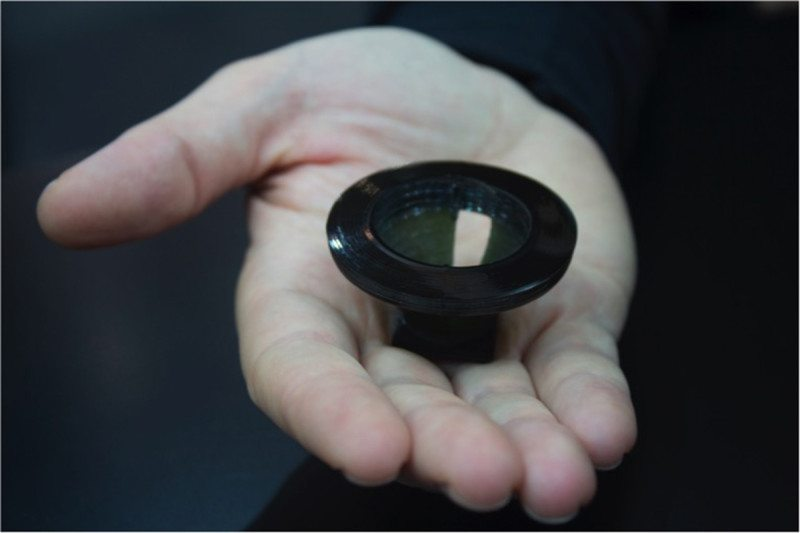
\includegraphics[width=\textwidth/2]{firstPrintedObject}
	\caption{First object made with AM.}
\end{wrapfigure}

	The first commercialized AM technology was Stereolitography (STL). There were experiments with curing layers of photopolymer resins simultaneously, thus creating separate layers. It was in Japan in 1981, when the first schematics of possible technology using photopolymer-hardening were described and proven to work. Later in 1984-1986, Charles Hull filed the patent for the first working machine\cite{FirstPatent}.
In 1986, he also founded “3D systems” company, which was probably the first company to do business with 3D printers. Nevertheless, Charles Hull is also important for his contribution to AM field by work on the “STL file format” – a specific format used by computers for describing the geometry of fabricated parts.\\
Technology that emerged later was Fused deposition modeling (FDM). This technology is using plastic material in a form of wire, which is molten and deposited into a single layer. The patent for FDM was filed in 1989 by S. Scott Crump from Stratasys Inc.  - also very important company in AM business that is still in operation \cite{CrumpPatent}.

	In the first half of 90s, remaining technologies were starting to be commercialized. They usually went under their specific names like "Selective laser sintering" or  "Laminated object manufacturing". These technologies were filling in gaps in missing technologies of "Powder bed fusion" (PBF), "Sheet Lamination" (SL), "Material jetting" (MJ) and "Binder jetting" (BJ) ; there is no need for naming all individual patents.
	
	When we mention patents and copyrights, we have to realize that patents have a major impact on development of AM. Technologies, processes and even materials from AM are subjected to patents. When patents are no longer held after 25 years, the competitiveness of other companies grows, resulting in bigger supply of AM machines and their price reduction. Expiration of patents was one of the reasons, why we experienced rapid growth of FDM machines.

\section{Comparison of AM and CNC machining}
%
Before I describe and categorize basic AM processes, it is important to see the distinction between AM and conventional CNC manufacturing. The reason being, both approach the same problem of manufacturing from different point of view. Fig. 2.2 illustrates this elementary difference.

	Conventional manufacturing processes are based on machining and processing block of raw material, thus it is \textit{subtractive process}. Using modern equipment, one is able to achieve very high precision of manufactured part with good surface quality. Materials such as steel and other metals are commonly utilized, alongside with plastics, wood and many other materials that can be processed. However, in general often parts of complex shapes could be very tricky to make. With CNCs, it is impossible to create objects with inner cavities or other internal features by machining the inside of the object. Also, machining shapes like curved overhangs or crevasses can be problematic. Furthermore, we haven’t considered the amount of waste material yet. Because we need block of raw material, exceeding the dimensions of the part made in all directions, it is not rare to machine away more than 80\% of material. This material then becomes waste material. Although scrap material is recycled, the blocks of raw material can be very expensive. Machining parts for use in aerospace industry might be a typical example. The parts are often of very complex shape, and made out of lightweight metals such as titanium. Requiring big block of titanium can be unnecessarily expensive - significant part of provided material in fact is unused and thrown away.
\begin{figure}[b!]
\centering
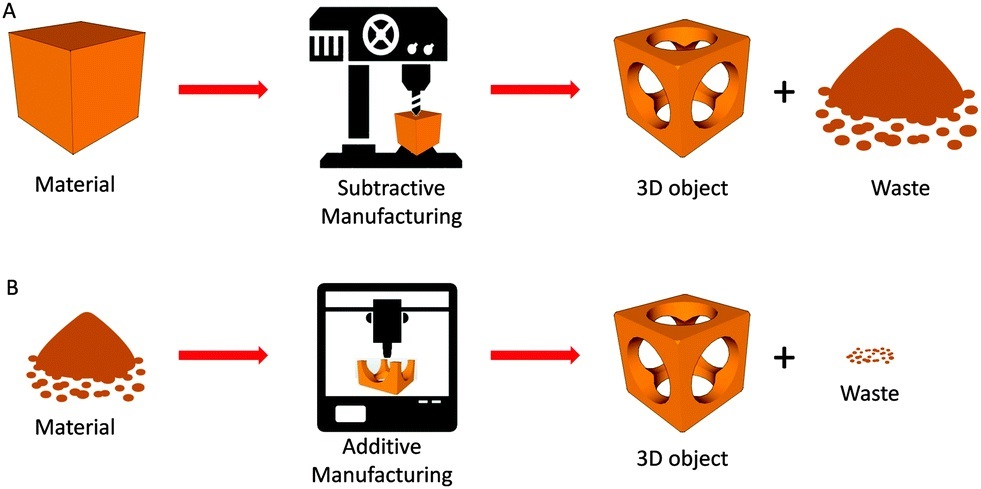
\includegraphics[scale=0.6]{additiveSubtractiveManufacturing}
\caption{Additive vs subtractive manufacturing illustration \cite{AdditiveSubtractive}.}
\end{figure}

	Another field of comparison of AM and conventional production processes is the scale and amount of produced parts. Conventional methods of machining are known for a long time, and are used for series production. The combination of CNC machining with i.e. mold casting is a fast and efficient process. Regarding these series-process chains, problems will occur when we want to alter a few manufactured parts. It is not suitable for making only few parts because of long preparation time, prototyping phase, and expensive equipment needed specially only for one kind of a product.

	As it follows from the name itself, AM is not subtractive, but \textit{additive manufacturing process}. Most of AM technologies are not limited by mentioned obstacles of CNC, such as manufacturing inner cavities or producing waste material. The simple idea, depositing material only where we want, results in having almost no waste material. Some technologies require material recycling though, but recycled material is immediately ready for use. Because AM machines are based on material deposition instead of removal, time of product manufacturing is almost independent of it's shape. In other words, AM machines don't care if we print a box, statue or a scaled model of a flower. The build time depends only on the amount of material deposited.

	This attribute comes very handy in production of single custom parts of complicated shapes. The example might be printing custom body-parts of implants, since they are always unique, person to person. Also, shape-free manufacturing comes very handy to designers, who used to encounter limitations of capabilities of conventional machines, making production of complex shapes tricky.
	
	For the comparison to be complete, it should also be mentioned that machining is often not suitable for processing hard and brittle materials. On the other hand, machining results in almost "isotropic part", if the material itself is isotropic. Meaning, there shouldn't be differences in machined part related to the direction of CNC tool movement. With AM, this is never the case - there is always some amount of unisotrophy, caused by building the part in different manner in Z-direction compared to X-Y directions.
	
	When we look at AM processes, we see a major difference - waste material is no longer a problem. When we want to produce small number of customized parts or objects, AM enables us to do so. The general process of object making (of course depending on specific technology) takes longer time, but considered that i.e. complex parts can be manufactured simultaneously in one go, they don't have to be moved from machine to machine. This may cause significant time savings, resulting in faster production process, even though the technology itself is not faster than CNC. Of course different technologies differ in build-speed.


\section{What precedes part production - AM process chain}
If we want to make use of modern AM machines, we have to be able to prepare everything necessary. Same as with other manufacturing  technologies, making parts using AM requires more or less preparation, and sometimes also post-processing is required. Let's look at the necessary steps, preceding or following the part making.\\
\subsection{Information about produced part}
If we take it from the very beginning, we have to start with knowledge of part to be produced. We have to know what we are building. This information is actually virtual model of a part. Virtual model in electronic form can be handled by computer and converted to other formats, which AM machines accept. There are more ways of creating virtual model of the part, but probably only two methods are used.
\subsubsection{CAD modeling}
When possible, it is obvious that creating model using CAD software can be the most efficient solution. When we use modern CAD systems, changing virtual model doesn't require much effort. It is very useful, if we are planning to make some changes with produced part - we are iterating and changing every version to make the part better. With CAD, it can be matter of a few minutes / hours to make new model and print it. With mass production tools, this process of iterations and changes of production tools (such as casting tools) can be very time and money-consuming.
\subsubsection{AM and reverse engineering}
It can also happen that we want to produce part, but we can't make use of CAD software. The part can be too complicated to create a model, and modeling would be inefficient. If we already have a part we want to build, i.e. we want to "copy" a real existing part, we can make a virtual model using some 3D scanning system or device. There are many devices on the market, enabling us to do so. Scanning devices vary in properties. Easiest criteria for their classification is to distinguish between contact and non-contact scanning devices. Examples of contact scanning device can be machines used in metrology for precise part measurement. Precision of several micrometers can be achieved.\\
%
\begin{figure}[h]
  \centering
  \begin{minipage}[t]{0.4\textwidth}
    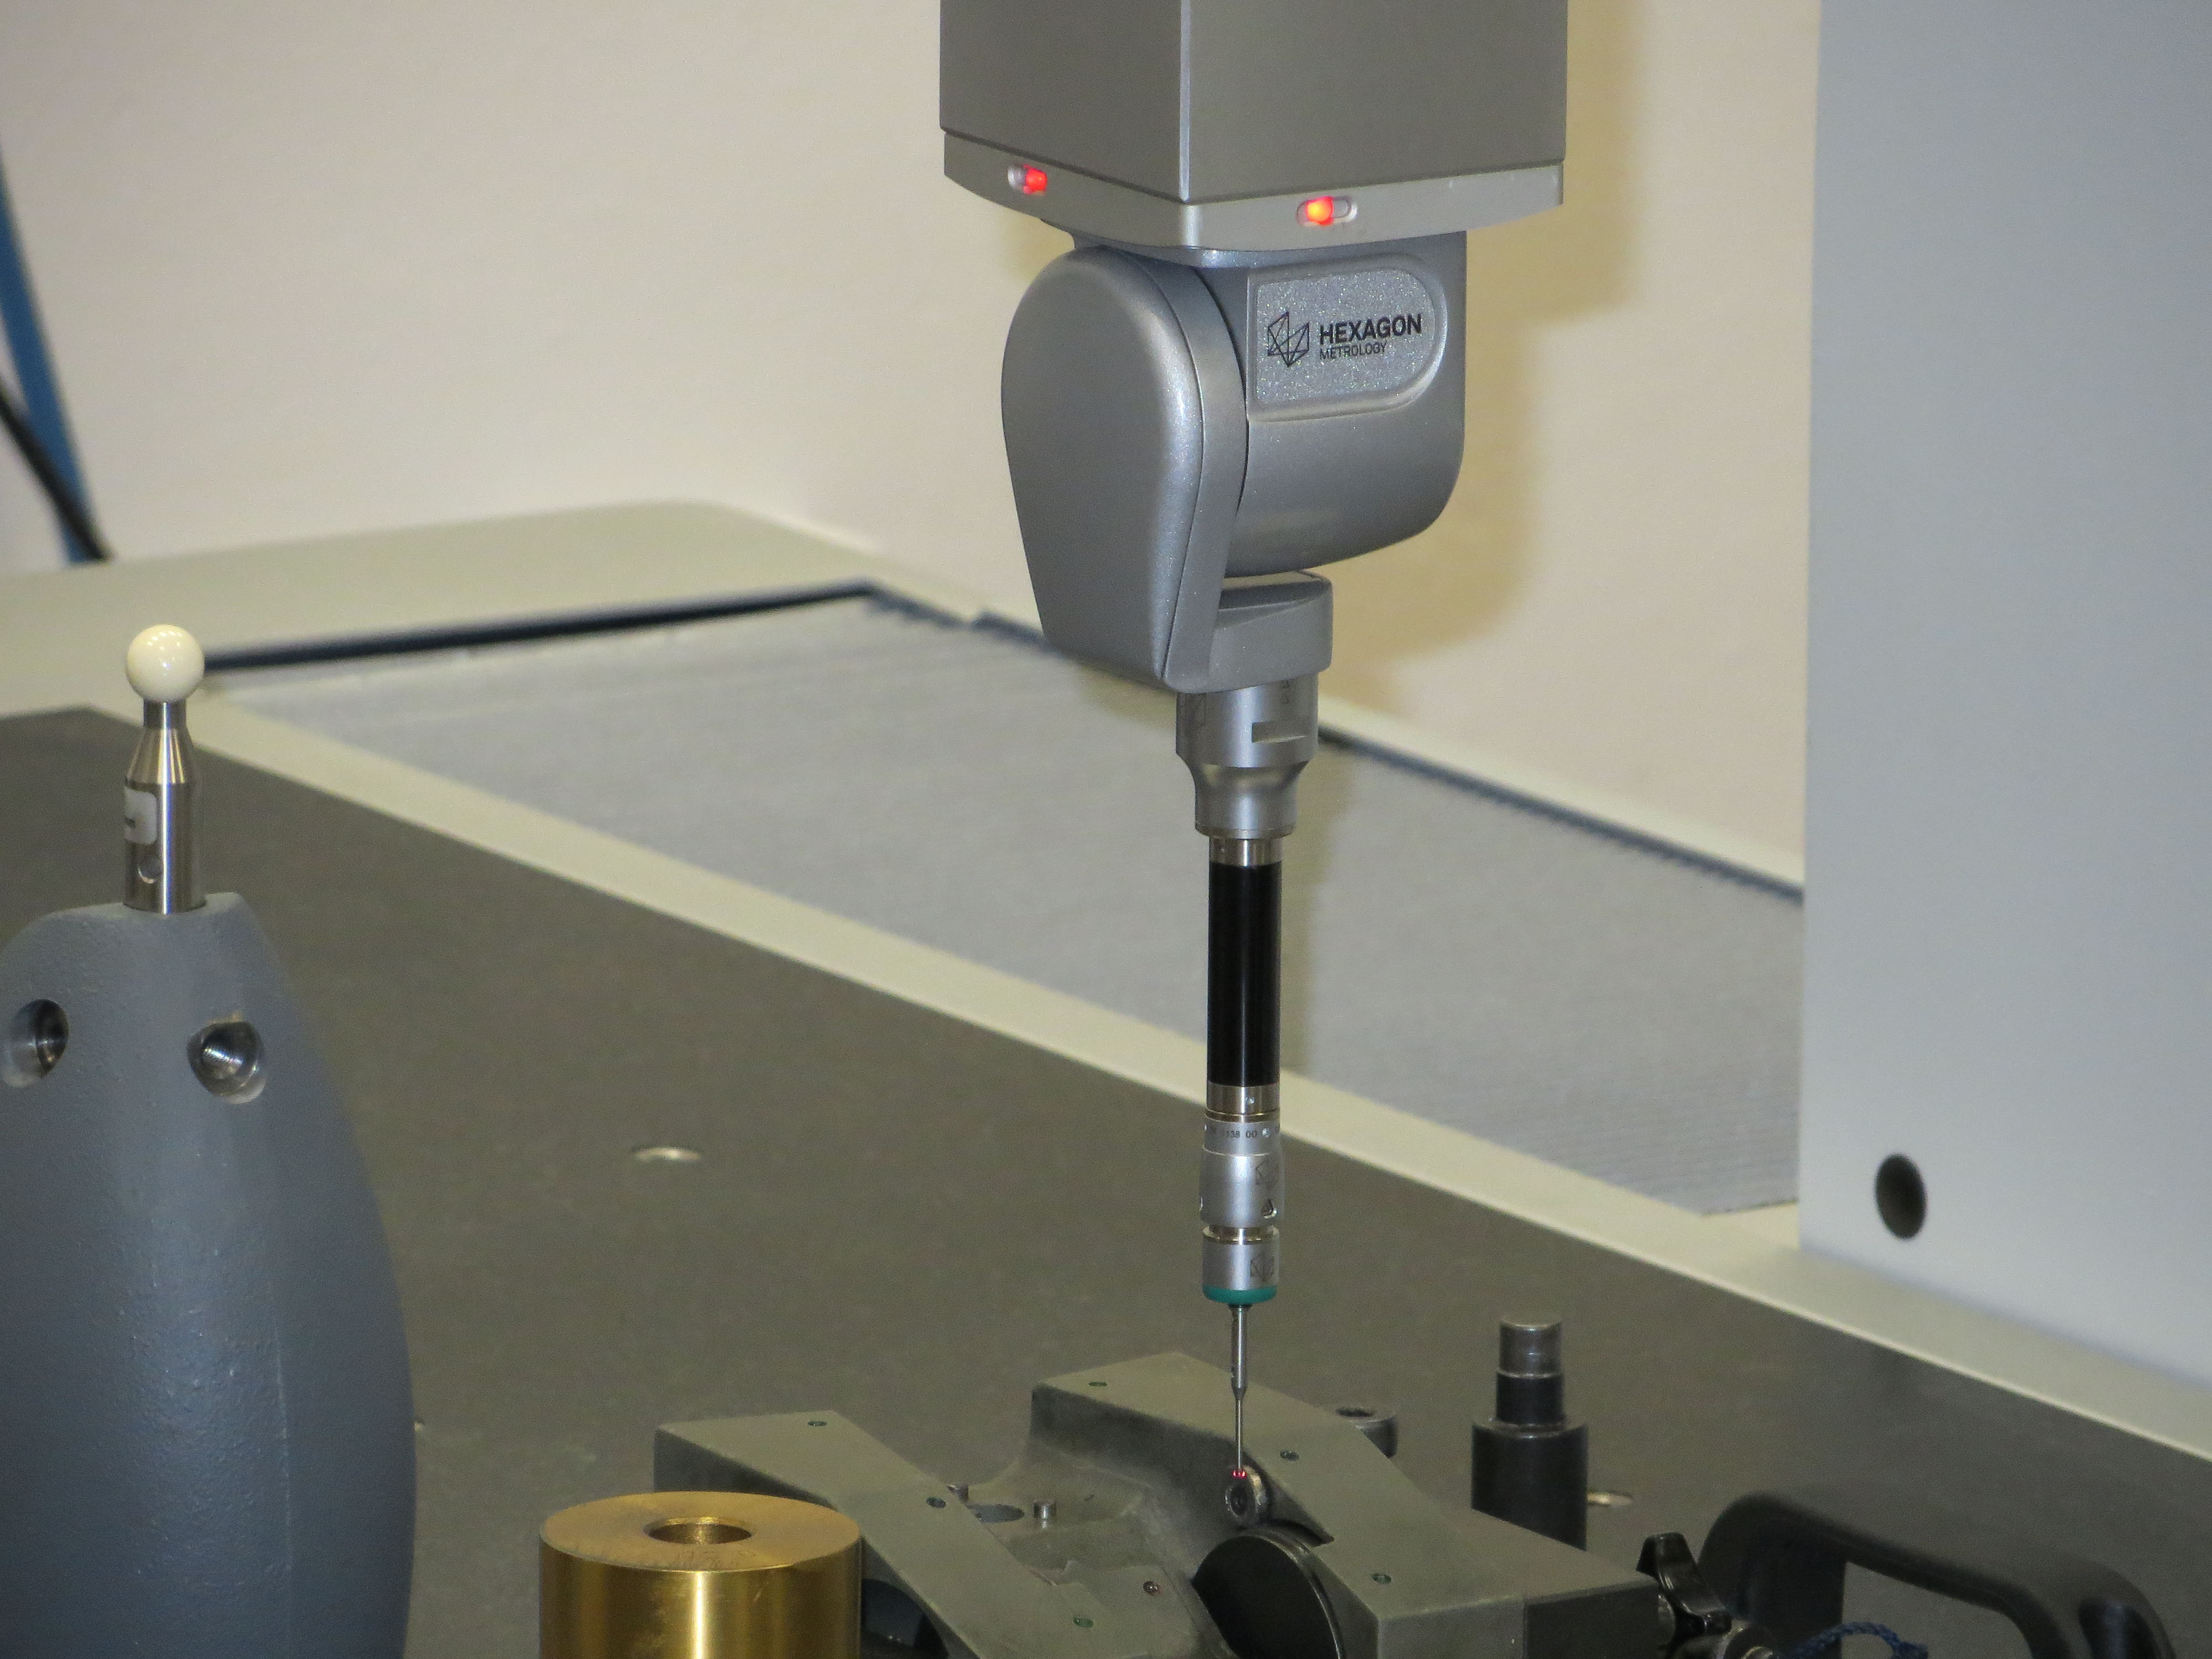
\includegraphics[width=\textwidth]{scanningMachine1}
  \end{minipage}
  \hfill
  \begin{minipage}[t]{0.4\textwidth}
    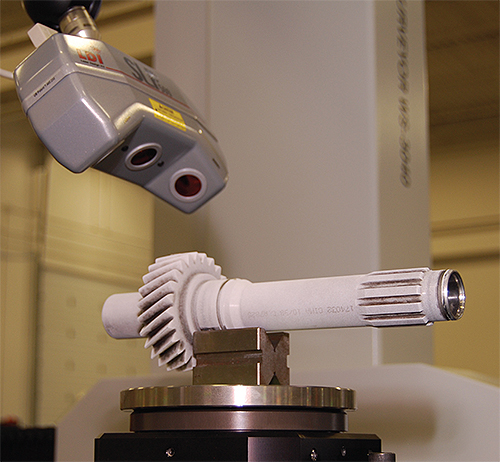
\includegraphics[width=\textwidth]{scanningMachine2}
  \end{minipage}
  \\[5pt]
  \begin{minipage}[b]{0.4\textwidth}
    \caption{Coordinate measuring machine}
  \end{minipage}
  \hfill
  \begin{minipage}[b]{0.4\textwidth}
    \caption{Non-contact laser scanning system}
  \end{minipage}
\end{figure}
%



    
Non-contact scanning devices vary in methods of measuring. Lasers can be utilized for distance measuring, or optical systems can be used. It is even possible with special photographic / optical software to obtain 3D model from multiple pictures of an object. Also, methods already utilized in medical field can be used - MRI machines or CT machines (micro-CT respectively) have been in use for several decades for medical purposes. Today, we can extend the use of these technologies, and use them as very precise scanning devices.
\subsubsection{File formats for AM software}
After obtaining the data, PC processing follows. Software for use with AM machines usually accept only specific data formats. The most common, that was already mentioned, is the "STL" file format.

	Although it is not essential to know, how the file format represents the geometry of the part, it can be useful to know, because it is possible that some glitches or errors can happen during processing. If we know the format specifics, we can guess where the problem can be. When it comes to "STL" file format, it represents the whole geometry with triangles - it creates a mesh of points on the whole surface of the part, and then connects the nodes to form triangles. That means if we want to accurately represent part geometry, with stl we have to have very fine mesh of points - The greater the distances between mesh nodes are, the bigger imperfections of the virtual model will be.
	
	STL file format is generally still accepted by AM machines, but it has some drawbacks. The biggest one is, the part geometry is the only thing it can describe. With modern AM machines, that is not enough, if we want to include additional information about the part in a single file. That is where additive manufacturing format - "AMF" file format comes in. AMF format enables us to describe, among other attributes, color of part for multi-color machines, material specification, or lattices and constellations within the part.
\subsection{Further data manipulation}
As expected, the AM machine itself doesn't accept nor "AMF" or "STL" file format. Since AM machine builds the part layer by layer, it only needs to know how to build each separate layer. Therefore we have to use software called \textbf{Slicer}. Each AM machine will have it's specification, but generally speaking, the output of the slicer should be a file with information, representing 2D shape of each layer. The machine itself then deals with the build process itself and starts printing layers - it doesn't care about their shape, it only deals with mechanics and kinematics of the building system.
\subsection{Machine preparation}
When the data are processed and ready to be sent to the machine, last remaining thing to be done before the build is the machine preparation. In some cases, there might be no need for any further preparation. With machines utilizing some kind of heat processing of material, preheating is often done. With PBF for example, preheating of the build space to high temperatures is done. Same with FDM machines, the metal extrusion nozzle is always heated to working temperature. Apart from preheating, some additional actions can be made, such as often crucial machine calibration or checking for any errors before build starts. Preparation stage is very important and shouldn't be neglected - small imperfection in the built part, caused by wrong machine preparation, can easily cause problems during the build process and ruin final product.
\subsection{Post-processing}
When we remove the built part, it might need some additional care to be ready for use. If building process heated the part, we usually wait until the part cools to ambient temperature to be processed further. Part removal is not always simple. With PBF technology, the excessive powder has to be removed and the part cleaned, usually by blowing pressurized air. Same with Stereolitography or Binder jetting, we have to clean the part from excessive photopolymer or powder respectively.

	If some support structures were added to enable the build, they also have to be removed mechanically. It is often done by hand, and it can involve honing, grinding and cutting. For many parts built with PBF or DED technology, there is residual stress in the part. Post-processing heat treatment is required to remove these stresses, caused by uneven heating and cooling and rapid temperature changes.
	
	With other technologies, post-processing can be desired, although not necessary - with FDM technology for example, where the final roughness of the part is not very good, manual grinding, polishing and painting can be done to improve the part appearance.
\section{Fields of applications}
As mentioned, there are several considerable differences between AM and machining part production. That's the main reason AM can be efficiently used in some fields more than others. The biggest advantages, such as shape-free production, ease of change of the model and speed of production in small quantities make it great for purposes such as prototype making, presentation product making, easily-produced life-sized parts (for visualization or testing), little waste material production and making products that won't be mass produced.\\
\subsection{Medicine}
There are many medical applications, either with medical instruments or with making prosthetic limb parts. Creating these isn't anything new joint replacement surgeries are several decades old \cite{JointReplacement}. Artificial joints can be made using CNC machines, and if made with AM machines, they will require post-processing - at least grinding and polishing to achieve perfect surface smoothness.

	But there is more to AM machines in medicine - apart from building replacements for body parts such as joints and skull replacement part, the technology can be used for printing specially designed surgical tools. Reason being, surgical tools can be very special, developed for only single type of surgery, therefore only few pieces of the equipment can be produced and mass production isn't appropriate.
	
	Illustrations of medical applications of AM are in fig. 2.5 and 2.6. Leg / arm plasters can be made too, designed to hold the limb in desired position and to be comfortable - built specifically to fit one's limb. Another example of combining AM with medicine can be custom printed teeth. There is machine available, that combines AM with 3D scanning procedure, and is capable of scanning patient mouth and printing custom tooth in very short time. \cite{DentalPrinter}. Not forgetting, customized hearing aids can be very handy - since everybody in need of hearing aid has different ear size and shape, shaping the outside frame of hearing aid can ensure that the final product will fit the customer perfectly. Last but not least, specific objects can be printed for medical educational purposes, so that students can practice performing sensitive  surgeries or interventions on models, accurately representing specific body part.
%
\begin{figure}[h]
  \centering
  \begin{minipage}[b]{0.45\textwidth}
    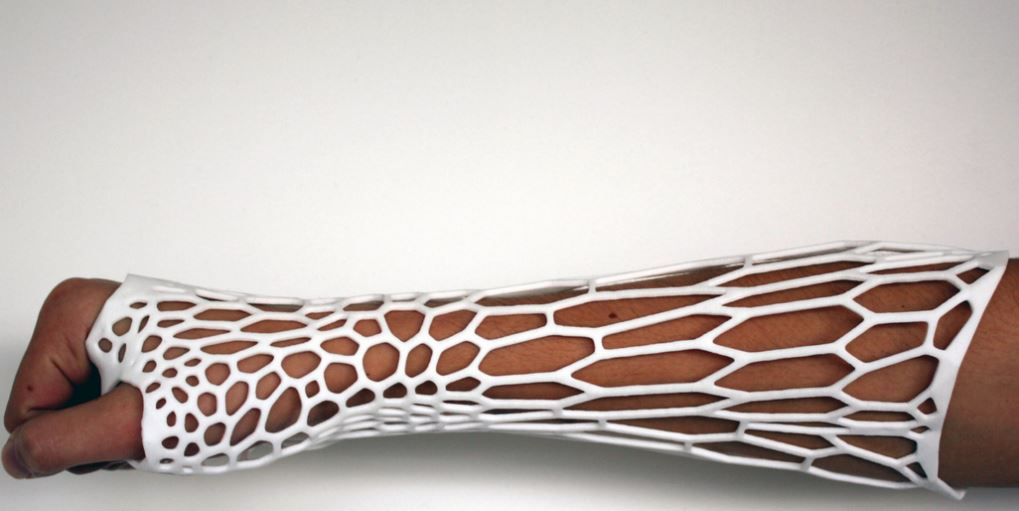
\includegraphics[width=\textwidth]{armPlaster}
  \end{minipage}
  \hfill
  \begin{minipage}[b]{0.45\textwidth}
    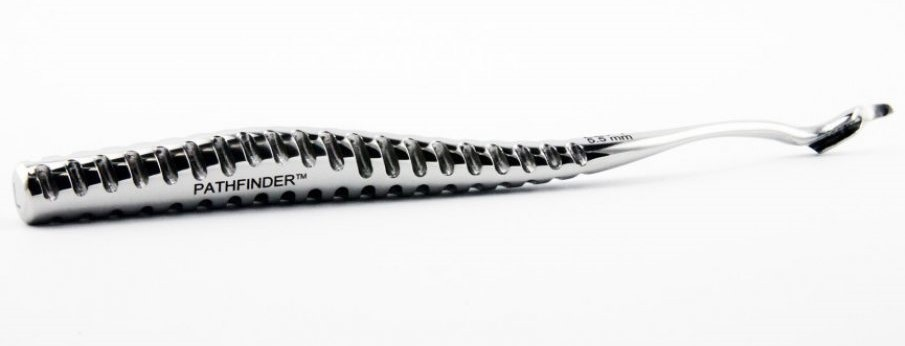
\includegraphics[width=\textwidth]{surgicalTool}
  \end{minipage}
  \\[5pt]
  \begin{minipage}[t]{0.45\textwidth}
    \caption{Arm plaster made with AM}
  \end{minipage}
  \hfill
  \begin{minipage}[t]{0.45\textwidth}
    \caption{specific surgical tool made using AM}
  \end{minipage}
\end{figure}
\subsection{Aviation industry}
Although AM is not primary production technology in aviation field, it can open great deal of possibilities. Many parts for aviation purposes are complexly shaped, and therefore complicated for machining. When a part from solid titanium block is machined to shape of i.e. turbine blade, it can mean that most of the material is machined away, even more than 80\%. Waste titanium can be recycled, but still the price of such titanium solid block is in range of thousands of EUR. When using PBF technology with titanium powder, we could eliminate the waste material, reducing the initial price of material. Still it is true that extra machining and polishing of such part would be required after, which could increase the costs, saved on material.
\subsection{Automotive industry}
Car production is, and probably will remain, thing of mass production. Yet, there is still place where AM can prove itself as useful. Before mass production, prototype making is again essential part, and therefore great deal of attention is always paid not to make mistakes during series preparation.

	Lightweight metals such as aluminum can be utilized for functional parts such as valves, canals or tubes designed for specific car type. Polymers also can be used for interior design, i.e. during stage of preparing "non-stressed" parts such as handles, coverings or panel parts - here AM can be handy for visualizing the interior.
\subsection{Architecture or design}
The reasons of AM being useful in this field is probably apparent from previous description - designers more than others can appreciate shape-free manufacturing, and not having to bother with limitations of conventional manufacturing. 
\subsection{Educational purposes}
This field might be found not as significant as others. Still, the fact is teachers and lecturers at high schools or universities could easily make use of AM during lecturing. For example, teaching biology or chemistry often require lots of teaching supplies, such as model of skeleton or models of chemical compounds to visualize chemical bonds. These supplies are often expensive, because there are not that many schools buying such supplies. Result is low demand for such items, and higher price - body part models can cost hundreds of EUR. With AM, teachers could only download / create desired model such as human organ or chemical bond model and print it, all that for fraction of the original price.
%
%
%
\chapter{Materials for use in AM}
The scale of materials usable for purposes of AM is very wide. We can today print objects from different plastics like Nylon, polystyrene and others. Objects can be printed out of common metals such as steel and it's alloys, titanium, aluminum and others. Certain technologies make it possible to print even sand parts. Other methods enable building colorful parts. Since there are so many materials, we should be able to categorize them into logical groups. Materials used with each technology will be described in detail in related chapters – this is only brief summary of material options.

	In following lines, some information might be slightly imprecise or misleading. The reason is, categorization of AM processes and related issues is very sophisticated and there are many slight differences among technologies. I will try to summarize some main ideas, but detailed description can be found in following chapters devoted to specific technologies.\\

\section{Material state}
One way of materials categorization is based on phase / physical state. Materials before printing process can be either solid or liquid. Solid materials can be used in forms of powder, wire or thin sheet / folia. Liquid materials are so far only photopolymers.
\subsection{Solid powder materials}
Powder materials are usually used for metal printing. Nevertheless, plastic and ceramic powders or sand might be used. Powder material can be processed by partially or fully melting and fusing together, creating a solid part with "Powder bed fusion" or "Directed energy deposition" technologies. Laser or electron beam can be used to melt the powder. Also, the powder can be glued by a special substance called binder (chap. 8 - Binder jetting). 
\subsection{Solid wire form materials}
Wire-form material is always used with "Fused deposition modeling" technology and rarely used with "Directed energy deposition". Within FDM, the plastic wire is partially melted and in controlled manner "spilled" and deposited. Due to its viscosity, one can precisely control the deposition process and it's precision. After solidification, plastic forms final object.
\subsection{Solid sheet form materials}
Sheet-form materials are used within the "Sheet lamination" technology. It uses thin sheet of metal, paper or basically any material, that can be cut and glued together. Each sheet equals one layer, that is cut into the shape of current cross-section.
\subsection{Liquid materials}
As mentioned, there are substances called photopolymers, used with AM. The principle is having a bath of photopolymer, which is precisely cured by light of specific wavelength. Where cured, material undergoes a chemical reaction, creating bonds between separate molecules and solidifying. "Stereolitography" of "Material jetting" commonly use photopolymers. In latter chapters, materials will be described more.\\
%
%
\section{Chemical composition}
We might also want to group materials based on their chemical composition. I will not fully describe chemical properties of materials like type of molecule bonds. Still, easily we can distinguish between main groups of materials.
\subsection{Metals}
Metals are generally materials that are good electricity conductors. This property is related to their other properties. Metals have generally higher yield strength (hundreds of MPa), very variable thermal expansion coefficient and medium-high melting point (important for heat curing of metals). They are also usually able to withstand some plastic deformation and do not absorp water.
\subsection{Plastic}
Other category is group of plastic materials. These materials have much lower yield strength, thus are not suitable for functional stressed parts. Usually they do not conduct electricity well and have low thermal conductivity coefficient, but higher heat expansion coefficient. Their melting / glass transition point is much lower than metal melting points, so they are easier to cure in this way.
\subsection{Ceramics}
Third category of materials used in AM are ceramic materials. Curing process is usually using ceramic powder. Melting point of ceramics is generally slightly higher than commonly used metals, but there can be exceptions. Ceramics is very hard and strong, yet brittle material. This property can be found problematic in AM. Because ceramics show almost no plastic behavior, they crack easily once they reach yield strength. This makes ceramics harder to process this way - during printing and for example heat sintering, rapid temperature gradients occur, causing thermal stresses and cracking.
\subsection{Photopolymers}
Among other materials are e.g. photopolymers. Even though they are plastic – polymers, I'd like to distinguish between them and other plastic materials, because they differ fundamentally in curing process. Default state of photopolymers is liquid, and it consists of more types of additives to make curing with light easier. Depending on point of view, they can therefore be considered different material from other plastics used in AM.
\subsection{Others}
Also, mixtures of different materials should be mentioned. Same we can make metal alloys of specific composition, we are able to incorporate small particles into plastic wires for FDM printing, like bronze of wood. If we have kind of material, consisting of 40\% wooden particles and 60\% polymer holding wooden  particles together, it is among one’s preference to say about which material are we talking about \cite{WoodenFilament}.
\section{Material processing}
Among other ways, we can also divide materials by the way of their processing.
\subsection{Heat processing} Some materials are processed by heat. They are fully or partially melted, and after cooling, material (like in most processes using metal powders) fuses or solidifies together into single physical object. Powerful lasers, or in case of conductive materials electron beam can be used instead as the heat source.
\subsection{Light processing}
On the other hand, liquid photopolymers are cured by light. Photons of specific wavelength (either UV, visible or other) initiate chemical reaction within material, causing creation of new chemical bonds and solidification.
\subsection{Other processing}
Binder jetting is the only technology, which basically doesn't process the material at all – it only binds the material together with special glue, called binder. There is no change of properties of the material, but the strength of the final part is limited by strength of binding particles, i.e. by the binder.\\
Also, with "Laminated object manufacturing" the sheets have to stick to themselves, which can be done using some special binding agent or glue.

\section{Common problems of material processing}
What we should realize when thinking about processing materials, are problems we are bringing along. Heat processes are related with thermal stresses, expansion / contraction and subsequent curling, warping and cracking. Similar issue is related to curing photopolymers, where curling and warping is caused not by heat, but by change of volume of material when changing state of matter. This is unique to binder jetting technology, which doesn't have to deal with these issues – as will be discussed in dedicated chapter.

	It is not always necessary to strictly distinguish between different materials. Instead of having fixed table of categorized materials, we should have complex knowledge of different kinds, their properties, pros and cons. 

\chapter{Photopolymerization}
Photopolymerization technology, also called "Vat Photopolymerization" or "Stereolithography" (hereinafter abbreviated as SLA), was the first introduced AM technology on the market. It utilizes ultimately photopolymers as default materials. Photopolymers were developed in 60s, yet SLA appeared aprox. 20 years later. Since then, SLA machines has improved, along with available photopolymer materials.

	SLA has many specifics of ongoing processes, resulting in both advantages and disadvantages of this technology. In this chapter, I will describe the general approach of this technology and relevant problematic, curing process itself, material properties and mention the overall conclusion of SLA.
\section{Basic operation principles}
SLA is no exception in relation to patent problematic - patents used to determine the direction of SLA development. That is not true anymore, since 25 years validity of most of relevant patents has recently ended. As some company patented some SLA specific approach, other companies had to come up with different solution to the same technical problem. Same applies for all other technologies, that can be newer and patents might be still valid. SLA is therefore versatile technology with SLA machines varying in many parameters. Among those parameters are build speed, machine reliability, precision, price and many more.\\
The biggest difference among SLA machines is given by different approaches to curing individual layers, as seen in fig 4.1. For now, let's summarize what all SLA machines have in common.

	SLA can also be called "Vat photopolymerization" because a vat is always present - a container, of which content is the photopolymer resin. Typically, the volume of the container is in range of several liters up to more than cubic meter of the resin - the amount of material it can hold. Above the vat, there is the source of radiation, used to chemically process the resin. This system, utilizing optics and other devices, is located above the vat so that it can be directed on the resin surface and cure the top layer of the resin.\\
The source of the radiation is also one of the parameters of SLA machines. Typically, machines utilize \textbf{UV light}, sometimes visible light, both in form of a laser. Other sources of radiation, such as electron beam or gamma ray, might be used. It also depends on the processed material - the ultimate condition for the curing process is that material has to undergo chemical reaction to solidify. All of these radiation sources can be used to deliver energy to the resin, and initialize the reaction. Again, used lasers / other sources can vary in terms of their power, spot size, material requirements etc.

\begin{figure}[t]
  \centering
  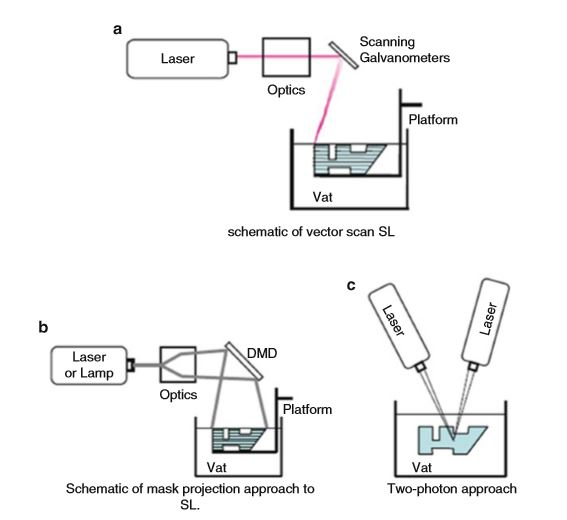
\includegraphics[width=0.8\textwidth]{SLAillustration}
  \caption{Illustration of SLA technologies, \cite[p. 65]{AMT}}
\end{figure}
%
\section{Curing process} 
It was mentioned that there are more approaches within SLA of how to cure a layer of the resin - the easiest sorting criteria for types of SLA machines. With these approaches described in following section, fig. 4.1 is added for illustration.
\subsection{Spot scanning}
The first approach is the most common one - layer is cured by a laser, which is projected onto the resin surface by mirrors (fig. 4.1a). Laser is focused in very small area, thus called spot scanning or point scanning. By changing the angle of the mirrors, we can control and move the location of laser spot on the resin surface. By constantly changing the mirror angles, we create a path - trajectory of the laser. When a laser moves past a point on the resin surface, it leaves solidified material behind - where the laser points, the material becomes solid. This approach is the oldest one and most of SLA machines utilize this approach.
\subsection{Mask projection with DMD}
Another approach utilize Digital micromirror devices - DMD to cure single layer at once. With spot scanning, curing a layer can take a lot of time, because the laser has to scan the whole cross-section surface, meaning the path the laser has to scan is very long. If we use DMD, we can speed up the process significantly. That is, because with mask-projection technology, we irradiate single layer simultaneously (fig. 4.1b or fig. 4.2).

	DMD is basically a 2D array of microscopic mirrors, that can be controlled and positioned individually. These DMD chips can have, for example, resolution of 1024x768 pixels, where each pixel represents a single micromirror. This micromirror can be switch between "on/off" state, so we can set a shape, that will reflect light, while remaining pixels will not reflect the light. Strictly speaking, we change the angle of the mirror between two positions, we don't turn the mirror off. When the light is projected onto the micromirror, we can control individual pixels - mirrors to control the shape, reflected onto cured layer. The light projected onto DMD, of course, has to be the kind of light photopolymer is sensitive to.
	
	With mask projection SLA process, we start by spreading a layer of photopolymer resin. Then, we set the DMD to reflect the shape of first layer, and then project light onto the surface, reflecting from DMD. After curing a layer, light source is turned off and next layer of resin is applied on the top of previous layer. Then, we set the shape of DMD to reflect the second layer and irradiate it. Repeating this process, we get a final part.\\
%
\begin{wrapfigure}{r}{0.35\textwidth}
 	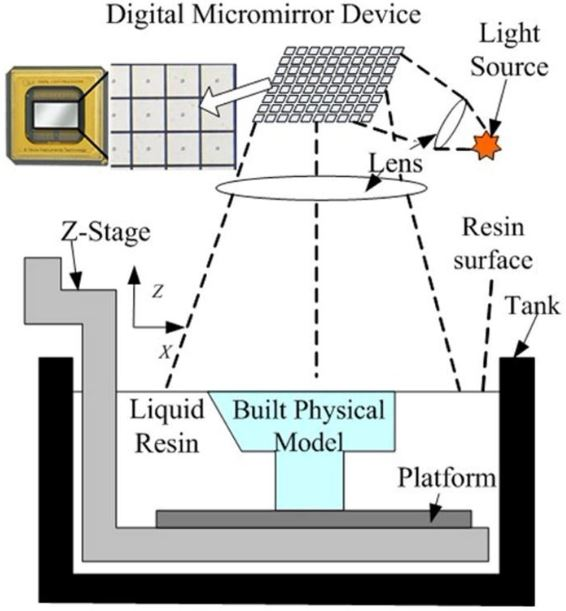
\includegraphics[width=0.35\textwidth, angle=0]{DMD}
	\caption{Utilizing Digital micromirror with SLA}
\end{wrapfigure}
%
The speed of mask projection is the biggest advantage. The general process of SLA can be sped up more than 10x compared to spot scanning. On the contrary, the limiting factor of DMD approach is the individual micromirrors size. Let's say we reflect the light from DMD to the surface of 20x20cm. If DMD has resolution of 1000x1000 pixels, then 1 pixel has resolution of 0.2mm. Such resolution would be very low and insufficient. In order to increase the resolution, we would have to either increase the resolution of DMD, or decrease the surface light is reflected to - make build area smaller. Higher resolution DMD can be costly and usually the resolution is lower than 3000 pixels on the longer side. The other solution, making build area smaller, is a obvious limitation itself.

	For the information to be complete, it should be noted that DMD is not the only device enabling shape projection onto the resin. Apart from DMDs, LCD display or spatial light modulator can be used. DMD is here used as an example for mask-projection approach.
%
\subsection{Two photon approach}
Third approach is very different from previous spot scanning / mask projection. It was developed for manufacturing very small and precise parts. Nowadays, parts smaller than 1 $\mu$m have been produced. More standard size of produced parts is in range of few up to tens of $\mu$m.

	The basic principle is, we have a small container of resin, and we direct two separate lasers inside the container. One laser is not enough powerful to cause the chemical reaction and solidification. This occurs only where the beams of lasers intersect (fig. 4.1c). Only in this very small region, that can be in ranges smaller than 100nm, the energy density is high enough to cure the resin. Due to this fact, the precision of built part can be greatly increased compared to other SLA approaches, at the expense of build speed. Also, there is no need for re-coating, since the process happens inside of the container, not on the surface, being another advantage of two-photon approach. The viscosity of the resin is usually high enough to prevent the part from flowing away before it is fully cured.
%
\begin{figure}[h]
\centering
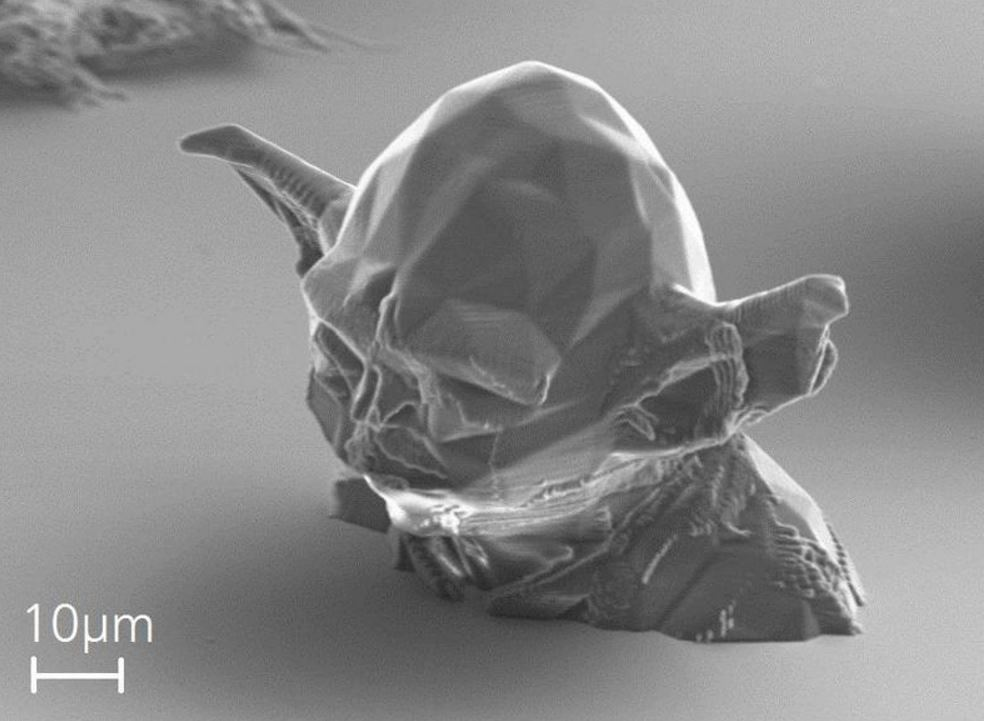
\includegraphics[scale=0.5]{yoda}
\caption{Image of a small statue of popular figure of YODA, made with two-photon SLA}
\end{figure}
%
\section{Photopolymer materials}
In this section, the \cite{AMT} is referring to \cite{SLAmaterials} as to primary source of following information on photopolymer materials.\\
\\
Different radiation sources used for resin curing were mentioned. From all of them, only light from visible or ultraviolet spectra is utilized within commercial AM machines; others remain in the field of research.

	As SLA uses polymers, they divide into categories of thermoplastic and thermoset polymers. For their properties only thermoplastic polymers are used. Thermoset polymers are unsuitable for SLA, since they can't re-melt.
	
	When we focus on thermoplastic polymers, we can put together list of material properties which determines how suitable the material is for SLA processing. Among others, we are often interested in reactivity / sensitivity to radiation, mechanical properties of the cured material (strength, brittleness) and amount of shrinkage due to phase transformation. The shrinkage is caused  by polymer molecules being smaller than  size of all previous uncured monomer molecules.
	
	Epoxy resins are used today. Before that, acrylate compounds were utilized. These two material categories have very different properties - acrylates tend to shrink more and are therefore difficult to process, but epoxy resins have slow reaction (photo) speed and are more brittle. Accordingly, often a mixture of these two groups is used to achieve desired properties of the final part.
	
	Among ingredients such as the epoxy resin / acrylate itself, the material mixture for SLA consists of more ingredients, which affect it's other properties. Namely, "photoinitiator, reactive diluents, flixibilizers and liquid monomers" \cite[p. ~67]{AMT} are usually present, where each constituent has a certain role. For instance, photoinitiator component works as a catalyst, helping to start the chain reaction and cross-linking of monomer molecules.
%
%
%
\section{Curing of materials}
%
\subsection{Theory and math of curing}
When talking about curing the resin to solidify, we have to consider the time factor - all individual processes during build take time. Same applies for curing - due to limited power of laser, speed of chemical reaction and other factors that can't be overlooked. In other words, we can't speed up the build process as we want, because curing processes themselves always take some time.

	When calculating basic build parameters, the most important parameter is the amount of laser energy, absorbed by the resin. There is critical amount of energy, which resin needs to absorb in order to undergo the chemical reaction. This parameter or energy per amount of material [$J/kg$] vary. With SLA, because of using finite layer thickness, this parameter is usually replaced by critical exposure with units of [$mJ/mm^2$], meaning critical amount of laser energy absorbed by 1mm$^2$.

	So we have to account for parameter of laser properties. Even though laser is focused into very small area, the energy density of laser vary in this area - energy density and exposure will be different in the center of the laser and at the edge.
	
	Following parameter, that also has to be remembered, is penetration of the laser. When the light hits the surface, part of the light will be absorbed in the form of energy, and the rest of the light will penetrate deeper into the resin. This results in different energy density and exposure, depending on depth under the surface. There is parameter called critical depth. Above this depth, for a given laser set-up exposure of the resin is high enough for the reaction to happen. Below this depth, laser light is too scattered and the energy density is below critical and no solidification will occur.


	All given parameters combined give us an equation, where the exposure of material is function of all spacial coordinates. According this function of exposure, we can border the region, where exposure is greater than critical exposure - the area where chemical reaction will occur. Outside of this region, the raw material will remain liquid, for the exposure was not sufficient. Because energy = power x time, with given laser power, there is minimal time the laser has to irradiate a certain place. For given laser power, we can calculate maximal build speed. From further mathematical equations used for description of ongoing SLA processes, it can be derived that a cross-section shape of cured line is a parabola.\\
%
\subsection{Scan patterns and other issues}
%
\begin{figure}[b!]
  \centering
  \begin{minipage}[b]{0.45\textwidth}
    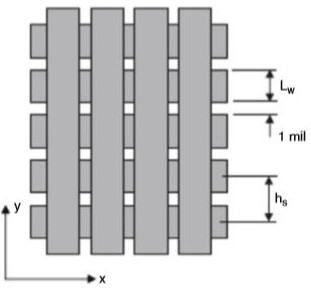
\includegraphics[width=\textwidth]{weave1}
  \end{minipage}
  \hfill
  \begin{minipage}[b]{0.45\textwidth}
    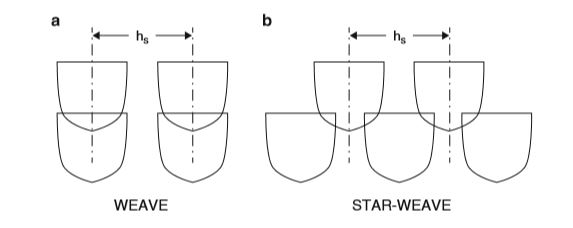
\includegraphics[width=\textwidth]{weave2}
  \end{minipage}
  \\[1pt]
  \begin{minipage}[t]{0.45\textwidth}
    \caption{Original WEAVE pattern, \cite[p. 87]{AMT}.}
  \end{minipage}
  \hfill
  \begin{minipage}[t]{0.45\textwidth}
    \caption{Comparison or WEAVE / STAR WEAVE patterns, \cite[p. 88]{AMT}.}
  \end{minipage}
  \\[10pt]
  \begin{minipage}[t]{\textwidth}
  \centering
  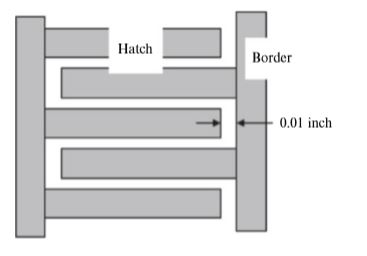
\includegraphics[scale=0.8]{retractedWeave}
  \caption{Retracted WEAVE scan pattern with improved shrinkage endurance, \cite[p. 90]{AMT}.}
  \end{minipage}
  \\[20pt]
\end{figure}
%
Even if we are able to precisely describe the curing process, it is not enough to secure a successful build. The curing process is happening on a small scale, but the overall build process brings other problems. For example, describing curing process doesn't account for shrinkage and residual stresses, anisotropic behavior caused by laser scanning trajectory, overlapping of cured lines, or layers sticking to previous / following layers.
	
	Problem of shrinkage and anisotropy of the build is interrelated. Simple explanation can be given by following example: We are curing a single cross section of full square. Let's say we cure the circumference of the shape first. Than, we have to cure the infill - inside of the circumference. One of the options is to cure horizontal or vertical lines, parallel to one of square borders. If we go from upper border to bottom border, than immediately after curing first upper infill lines, the upper part of square will tend to shrink. This will cause either decreasing dimension of the square, or internal stresses which will remain.  By this simple approach, we are causing anisotropy, since we have a scanning pattern preferring a single line direction. This issue we can try to eliminate by curing next layer perpendicular to previous one. By switching the pattern, to some extent, we eliminate the anisotropic property of the build - the build as a whole is more or less isotropical, but individual layers vary from each other. Also, we should bear in mind, that if the part shrinkage is problem not only for causing stresses, but also for changing dimensons of the part. The resolution of SLA printer can be in range of tens of microns, so even if the shrinkage will not ruin the build, we might not be able to stick to our desired part dimension - the real part built might be smaller due to shrinkage.
	
	Problem of overlapping layers is, that we have to irradiate more energy to the resin than the critical exposure. Reason being, the current layer has to cure into previous layer. This re-curing of previously cured layer requires some additional energy, by which critical exposure has to be increased, decreasing theoretical maximum build speed. However, this overlapping also causes deflection of already cured sections, and adds another source of anisotropy to the build.
	
	To account for all of mentioned and other related issues, certain scanning patterns for SLA were developed. Here, by scanning pattern is meant how the infill of layer circumference is cured. These scan patterns are called WEAVE and STAR-WEAVE. Further improved comes the retracted hatch WEAVE scan pattern. Illustrations of these patterns are in fig. 4.5 , 4.6 and 4.7. With these scan patterns, negative effects of SLA builds can be minimized for securing successful build.

%
\section{Conclusion}
All necessary being said, let's summarize the pros and cons of SLA technology.
%
\begin{itemize}
\pro \textbf{Part precision}\\
Not only with two-photon approach, we can achieve parts of high precision, to which only some other technologies are comparable.
\pro \textbf{Surface finish}\\
Surface roughness is incomparably better than of parts made with e.g. DED or FDM technologies.
\pro \textbf{Build speed}\\
Although build speed is a relative term and depends on build set-up and parameters, SLA is often quicker than other technologies.
\\[10pt]
\con \textbf{Support structures}\\
Need for support structures is present with SLA. When machine operator removes the built part, it requires cleaning from the resin, and often mechanical removal of the support structures.
\con \textbf{Materials}\\
As the term photopolymerization implies, range of available materials is limited to thermoplastic polymers.
\con \textbf{Price}\\
Furthermore, same as SLA machines themselves, these materials are often very expensive. Single liter of the resin can cost hundreds of EUR. With biggest nowadays SLA machine, even filling the container full can cost thousands of EUR. The price of big machines, able to print more than 2 meters wide objects, can be higher than 500 000 EUR.
\end{itemize}




\chapter{Powder Bed Fusion}
Powder bed fusion (hereinafter "PBF") is counted among the oldest technologies commercially introduced. It can utilize variety of materials and final products can be fully dense functional parts. PBF is in some aspects of part manufacturing superior not only to other AM technologies, but even to CNC machining.\\
	The trade-off for it's abilities and versatility is in the need to understand all simultaneous processes during PBF printing, and need to set all print parameters carefully. Also, post-processing of the part is required, unit for recycling the powder is needed and other supplementary equipment (Oven for heat treatment, machine for infiltration) might be necessary. Machines themselves, materials and the overall machine maintenance and operation is generally expensive.

\section{Basic operation principles}
As follows from the name, PBF uses material in a form of \textbf{powder}. Although very simplified, we can say that any material in form of small particles, that can be melted together can be used (chap. 5.3 - materials).\\
	There are many types and variations, distinguishing different PBF machines. For example, single machine is usually not capable of processing any material, but rather only polymers or metals. Also, different machines might utilize other heat sources to cure the powder, or use different powder handling mechanism. So, even though the main principle for all machines is the same, the mechanisms utilized by various PBF machines can vary significantly.
\\
\begin{figure}[b]
	\centering
 	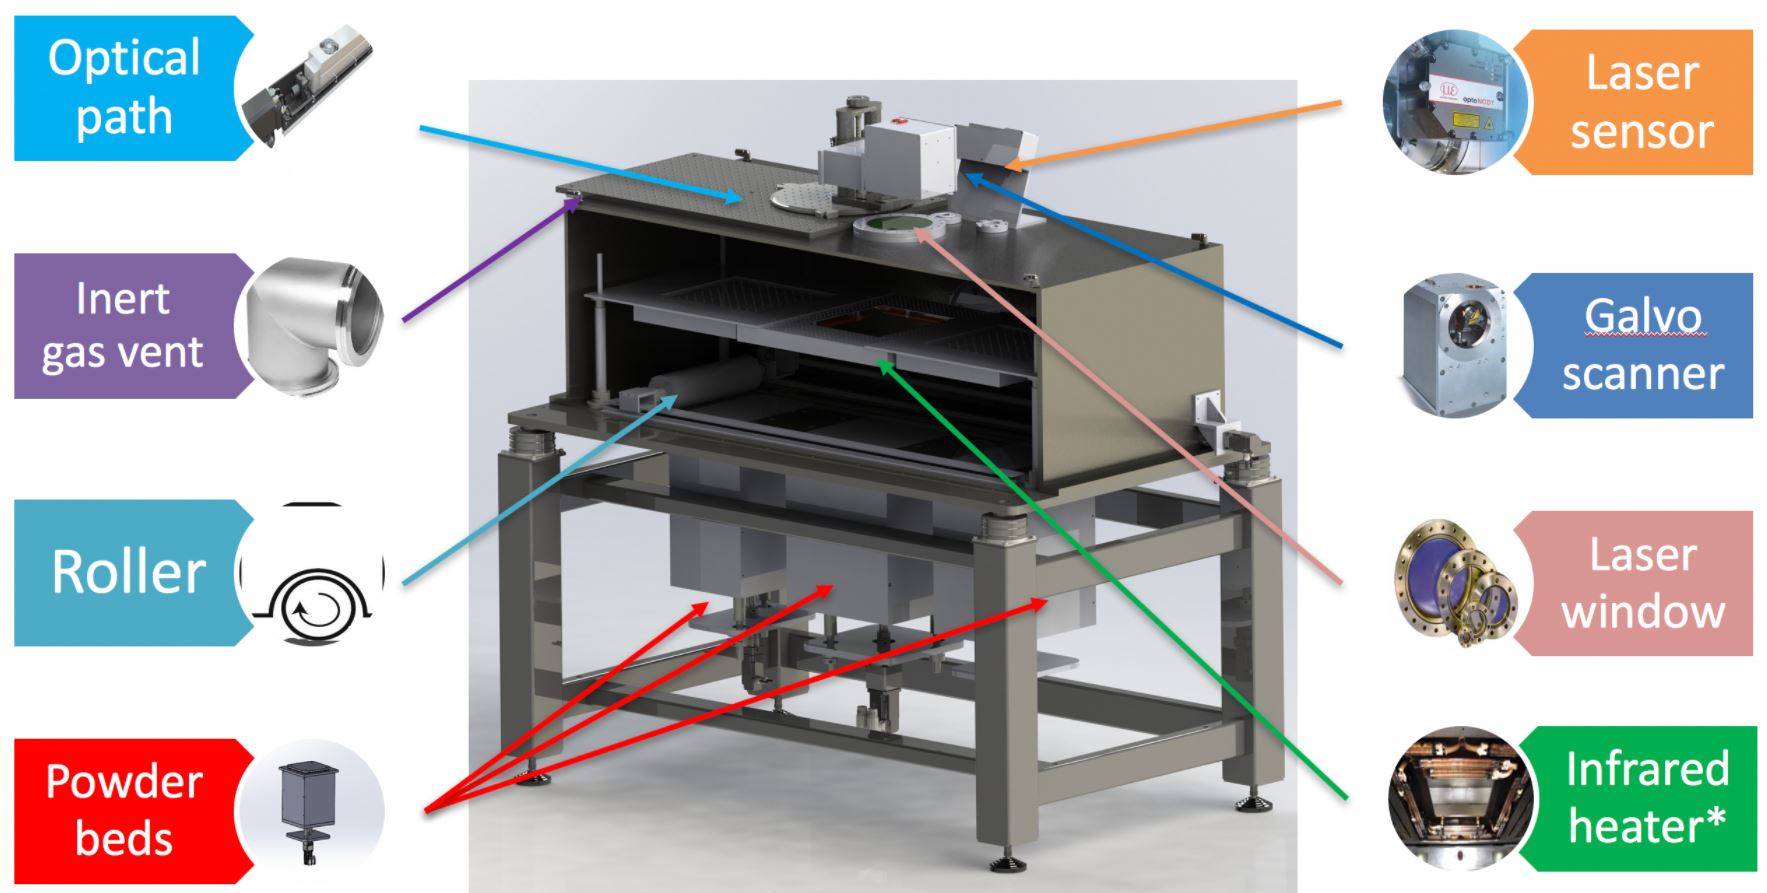
\includegraphics[width=0.8\textwidth]{PBFMachine}
	\caption{Real PBF machine, showing all necessary utilized equipment, \cite{unconn} }
\end{figure}
In the fig. 5.1, we see a typical PBF machine setup. The powder is held in a \textbf{container}, that might be heated. The \textbf{build platform} is the place where the actual part is built. When a current layer is cured, the build platform is lowered by one layer thickness, and new layer is moved from the powder container and spread onto the build platform by \textbf{spreading mechanism}. The newly spread powder has to be uniformly and precisely leveled and packed. The cross-section of layer is cured together - \textbf{melted or sintered by heat}. The process of layer deposition and curing is repeated until the part is finished.

	After the whole part is built, it has to \textbf{cool down slowly} to prevent uneven cooling and resulting curling. After cooling, the part is removed from the powder and post-processed - residual powder is washed away, support structures are cut and part can be machined or polished to achieve good surface finish. \textbf{Support structures} are not necessary since loose powder supports newly deposited layers, but they might be desired to hold the part in place due to rapid cooling rates and thermal stresses, that might cause warping and curling.
	
	Apart from finishing post-processing, part infiltration might be needed to achieve a dense part, if part porosity is too low. For part infiltration, same as with "Binder jetting" (where pores might be bigger), liquid metal like copper might be used. Although iron is not used with PBF, \cite[162]{LPS} mentions infiltration process of porous iron with copper infiltrant, and also mentions using silver as an infiltrant, and probably way more metals can be used for infiltration to fill material pores.
	
	The whole build space is generally \textbf{held at elevated temperatures}, usually as high as possible below the melting point. \textbf{Inert atmosphere or vacuum} is needed to prevent the loose powder degradation of electron beam diffusion (chap. 5.2.2 - heating methods). Pre-heating the powder significantly lowers the energy, required to reach the melting point and sinter or melt the material, reducing required heat source power.
	
\section{Powder bed fusion variations}
Although all PBF processes share the basic approach, we can categorize them based on utilizing different mechanism to perform certain tasks.

\subsection{Powder spreading}
When a current layer is cured, the build platform lowers by one layer thickness and new layer of powder has to be spread over the previous one. The powder is first deposited on the top of previous layer and then leveled.

\subsubsection{Counter rotating roller}
Roller, which is a part with shape of an ordinary cylinder, is rotating and simultaneously moving sideways - it is best illustrated with fig. 5.2. This method easily allows changing the layer thickness and the related packing density of the powder, by moving roller up or down.
\begin{figure}[b]
	\centering
 	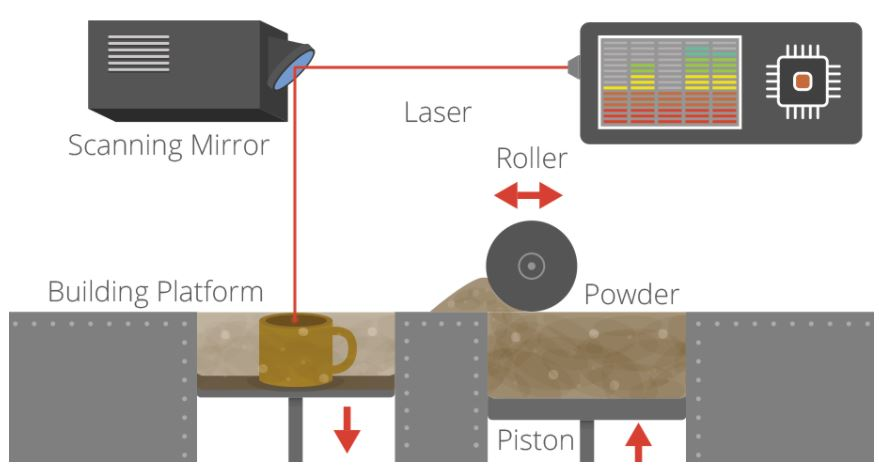
\includegraphics[width=0.6\textwidth]{roller}
	\caption{Illustration of roller spreading mechanism, \cite{chinese} }
\end{figure}

Also, by rotation counter the sideways movement, the roller "fluidizes" the powder during spreading - the powder "flows" before the roller, which significantly reduces the shear force acting upon previous layer. This is important not to disrupt stacked layers of powder.
\subsubsection{Blade leveling}
As it follows from then name, this approach utilizes a blade, which is just very thin and precise strip of metal, that is used to precisely level the layer and remove excessive powder. However, this method applies greater shear force upon deposited powder. The reason for using this method might have been the fact that roller mechanism was patented and therefore limited commercial use.

\subsection{Heating method}
This subsection discusses possible methods, how to heat the powder to cure and bind it together. Lasers are most commonly used as the heat source, but electron beam ("EB") is another option.
\subsubsection{Laser}
Laser is a beam of photons. With PBF, when photons hit the powder, some of them get absorbed by powder particles, converting their energy to heat. Both polymer and metals, eventually ceramics, can be cured by laser, but there are big differences in properties of polymers and metals, requiring different laser power, speed of laser scanning, spot size and other parameters. Different types of lasers are utilized with ongoing research and development in field of lasers (CO2 or Nd-YAG lasers, replaced by fiber lasers etc. \cite[p. 252]{AMT})

\subsubsection{Electron beam melting}
The electron beam melting process ("EBM"), developed at the Chalmers university in Sweden, utilizes an electron beam, which is focused onto the powder and fuses it together. When electron beam hits the powder, kinetic energy of electrons is transformed to heat. Compared to especially laser processing of metals, EBM is much more efficient process in terms of delivering energy to the powder (or used to be, due to low efficiency of past lasers with power-light converting efficiency of 10-20\%). However, EBM uses only materials with \textbf{high electrical conductivity}, so it can't process polymers or some metals with insufficient conductivity.\\
\begin{figure}[h]
	\centering
	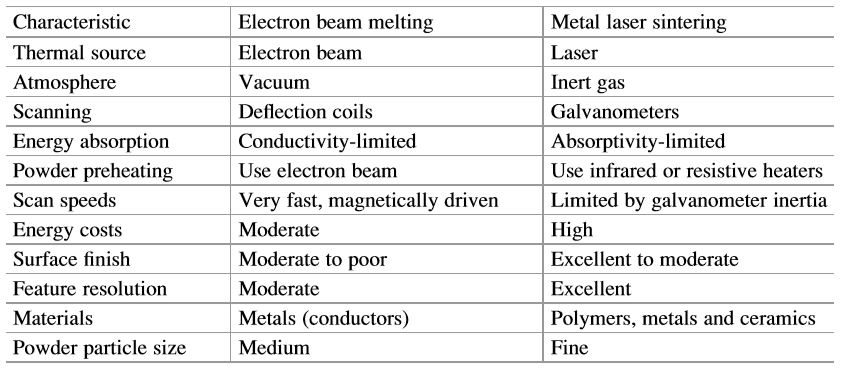
\includegraphics[width=0.9\textwidth]{EbmMlsDifferences}
	\caption{EBM vs. metal laser sintering differences, \cite[p. 137]{AMT}}
\end{figure}
	The need for very high conductivity follows from the \textbf{law of electrostatics}, saying that particles having the same charge repel each other - if neighboring powder particles are both charged, the repulsive force can overcome gravitational and other forces and the powder might disrupt. Also, charged powder would repel the incoming electrons coming from the electron beam, making the electron beam more diffused.\\
	The results of EBM properties and process specifications, compared to laser curing, are limited range of usable materials, and less precise parts with worse surface finish and bigger grain sizes.\\
	On the other hand, an advantage of EB is lower cost over a laser system of equivalent power. Also, electron beam is focused and controlled much more easily compared to laser - electron beam is focused by two perpendicular anodes surrounding the beam, that and controlled by electricity, enabling almost instantaneous beam controlling and scanning. The laser beam, however, is usually controlled by mirror galvanometers, which have some inertia, making laser scanning process slower than EBM processing.
	
\section{Materials for Powder Bed Fusion}
Variety of materials can be utilized with PBF, including \textbf{polymers, metals, ceramics and composites}. In theory, any material able to melt and solidify more than once can be used. Reason being, when the layer is being cured, the previous layer has to partially re-melt to be cured together. From polymers, \textbf{thermoplastic polymers} are suitable compared to thermosets, which can't re-melt. Also, polymers with crystalline/semi-crystalline structure are preferable for their distinct melting point, compared to amorphous polymers, that don't have specific melting temperature and are more suitable for material extrusion.

	With metals, situation is different. Usually, if a metal \textbf{can be welded}, it is supposed that processing it with PBF should be possible. There are however different problems that those with polymers. Compared to polymers, metals tend to oxidize and have much greater optical \textbf{reflectivity}, making metals more difficult to process via laser. That is especially true for case of processing aluminum - it has very high reflectivity and doesn't absorb much energy, so only some alumina alloys are available for PBF processing. Also, because of higher melting point of metals, lasers of higher power are used. Lastly, metals also have significantly higher \textbf{heat conductivity} compared to polymers and \textbf{higher surface tension}, resulting in different handling and processing.
	
	Since material is powder, the specification of the powder it has to be taken into account. In other words, powder properties, such as \textbf{particle size range and particles shape} affect the process. Fine powder is more appropriate for creating fine features, but requires more careful handling (chap. 5.5.1). The particle size has to be smaller than layer thickness for a single layer to be uniform. Typical values of powder particles are in range of units or tens of microns.
	
	To give an example of utilized metals, PBF can process commonly stainless steel and other steel alloys, titanium alloys, cobalt-chromium and possibly aluminum alloys.
	
	Finally it can be said that PBF machines utilizing polymers will probably have different architecture that machines for metal processing. Machines that would be able to cure both types of materials would likely face too many problems to be commercially successful.

\section{Fusion mechanisms}
Taken from \cite{AMT}\\
Raw material in form of powder has to be bound together to take the final part shape. There are 4 different methods of  fusing the powder together.
\subsection{Solid-state sintering}
With solid-state sintering, powder is bound together at elevated temperatures, but without melting. The temperature of the powder is held below the melting point, and binding process is driven by \textbf{diffusion}. At enough elevated temperatures, even though powder particles are not molten, 2 powder particles that have a small contact area are driven to fuse together to lower the total surface energy.
During fusion, necking between particles starts, and as the process continues, particles are fused more and more, lowering their total surface area and surface energy, getting into more stable state.\\
\begin{figure}[t]
	\centering
 	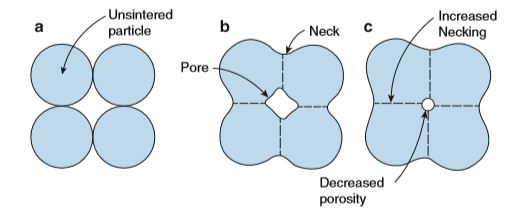
\includegraphics[width=0.8\textwidth]{necking}
	\caption{Illustration of particle fusion and necking process, \cite[p. 113]{AMT} }
\end{figure}

\subsection{Chemically-induced sintering}
With chemically-induced sintering (or chemically-induced binding), the binding of powder happens because or a \textbf{chemical reaction}. Such reaction is locally activated by thermal source - as a small region is heated, higher temperatures allow the reaction to take place by giving it enough activating energy.

	The chemical reaction can happen between either the powder and surrounding atmosphere, or between two powder particles, that are previously mixed as default powder material. For reaction between powder and atmosphere, \textbf{oxygen or nitrogen} are usually the gaseous reactants. Common characteristic of chemically-induced sintering method is higher part porosity.
	
\subsection{Liquid phase sintering}
\begin{wrapfigure}{r}{0.6\textwidth}
 	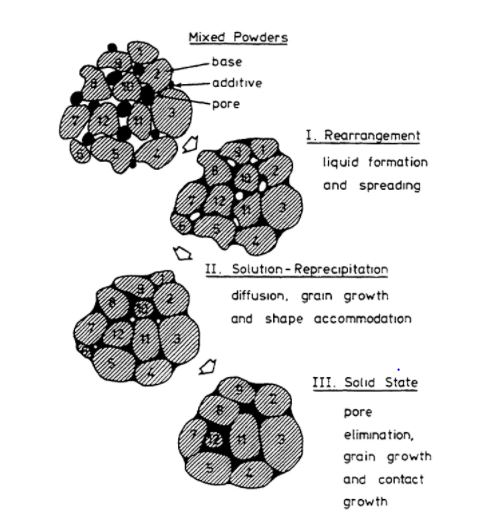
\includegraphics[width=0.6\textwidth]{liquidPhaseSintering}
	\caption{Liquid phase sintering of separate particles mixture, \cite[p. 6]{LPS}}
\end{wrapfigure}
Liquid phase sintering utilizes a powder, where 2 or more types of constituents are present. The purpose of multiple compounds presence is, that one constituent in the powder acts as a binder which melts, while the other constituent remains solid, acts as structural material  and is bound by molten binding constituent, which acts as a glue to hold and form the part.

	There are 3 ways how to mix binding and structural material into mixture.
	
\subsubsection{Separate particles}
A powder is simply a mixture of binder particles (melting) and structural material particles (not melting). Such mixture has to be well mixed. For both constituents, their volume ratio and size of the particles ratio is an important factor that determines properties of the final part.
\subsubsection{Composite particles}
Powder consists of particles, that are composed of 2 different constituents - the binding and structural material are both present in a single powder particle. Examples might be particles consisting of polymer and metal or ceramic, with polymer portion acting as a binder and metal / ceramic as structural material. It is also possible to mix two metal materials, where the one with lower melting-temperature acts as binder and the other one as structural material.

	The advantage of composite particles for PBF is that the resultant parts are more uniform, tend to have better surface finish and be of higher density compared to separate particles mixture. On the contrary, manufacturing such composite particles is more difficult than simply mixing two powders, which makes this kind of material more expensive. Typical example of composite particle material is nylon, filled with small glass beads.
\subsubsection{Coated particles}
Coated particles are a different form of a composite particle - a single particle of structural material is \textbf{coated with a binder compound}. This method of binder-structural material combination has advantages primarily of high absorption of the laser and more efficient binding.

	High absorption of binder agent is very important - for improperly chosen structural and binder constituent, it could happen, that the structural constituent might have significantly higher absorption rate and higher thermal diffusivity, which would cause the structural powder to melt prior to the binding constituent, despite the fact of having higher melting temperature. Also, because only binder is absorbing the energy from the surface, the coating melts first and the structural particle is not affected by heat much, resulting in better binding. Last but not least, since binder is coated on the particle surface, when molten, it improves the binder ability to flow. In comparison with particles mixture, when separate structural/binder particles are heated, even though the binder is molten, due to it's viscosity it might not flow fast enough to properly bind the structural material.

\subsection{Full melting}
Full melting is probably the simplest principle of mentioned processes - a small region of powder is heated, resulting in full melting of that region and creation of melt pool. When the heat source is focused on different region, the melt pool almost instantly solidifies. Because of rapid cooling rates of melt pool, unique micro-structures with small grain sizes can be created.

\section{Other problematic}
There were already some problems mentioned, like reflectivity of metallic materials. However, except of material-specific problems, general process of using PBF machine can face other complications.
\subsection{Powder handling issues}
One of the biggest challenges of PBF is problem-free handling of powder material. When spreading the powder, correct amount of powder must be spread over previous layer, that has to be smooth. As was mentioned in section about different leveling mechanisms, the shear forces upon previous layer during spreading has to be minimal not to disrupt layers.

	Related problem is, as size of powder particles decreases, the powder tends to loose the ability to "flow" and electrostatic charging with friction between particles starts to play a big role - with finer powder, it is more difficult to handle and spread it. When handled improperly, powder particles can become airborne and float because of the same electrostatic charge of neighboring particles.
	
	However, in order to create fine parts with small features, as fine powder as possible should be used. Therefore, in the end it is question of compromise between part quality and ease of powder handling.
\subsection{Elevated temperatures of unprocessed powder}
As was mentioned, powder within the build platform is held at elevated temperatures, often as high as possible below the melting point, to make the processing easier. However, as follows from principle of solid-state sintering, an important side-effect of pre-heating is that, when exposed to high temperatures, even the unprocessed powder is that even the unprocessed powder can partially sinter together, even though not desired, and can't be easily recycled.
\subsection{Material recycling}
Related to previous problem, material recycling is an important part of PBF process, since available materials are expensive. We want to recycle as much powder as possible, but some powder unintentionally sintered can't be re-used straight away. Also, even if the unused powder doesn't sinter together, after long temperature exposure it might change it's properties, making the recycling even more complicated. In order to secure repeatability of the print, the powder during each print has to exhibit the same properties. To achieve such print-to-print uniformity, unused powder is mixed with partially used powder in different ratio, depending on thermal profile used powder was exposed to and other used-powder specifics.

\section{Conclusion}
\begin{itemize}
\pro \textbf{Available materials}\\
Variety of engineering-grade materials are available for PBF processing, making PBF perfect for rapid tooling, prototyping and end-use part manufacturing.

\pro \textbf{Flexibility, support structures}\\
PBF in istelf is very flexible technology, that if handled properly, can produce parts of very complex shapes, difficult to create even with other AM technologies. Support structures are not needed to support next layer of powder - loose powder serves as a support.
\\[10pt]

\con \textbf{Support structures for warping (not EBM)}\\
It can happen, that the shape of produced part needs support structures to prevent curling and warping due to uneven cooling and thermal stresses.

\con \textbf{Time}\\
Because the laser is able to cure the layer only at one point at one moment, the printing process for PBF can be very long. Build times can be shortened by using more lasers to cure a layer at different places simultaneously.

\con \textbf{Price}\\
Because of all necessary equipment and features, PBF machines are very expensive, costing even millions of EUR.

\con \textbf{Post-processing, accuracy and surface finish}\\
Compared to flexibility regarding available materials, surface finish and precision of PBF produced parts is not great. Apart from removing possible support structures, it may require additional post-processing to improve the looks or achieve dimension tolerances.
\end{itemize}




\chapter{Material extrusion}
Technology of material extrusion (also Fused Filament Fabrication - FFF, or more commonly Fused Deposition Modeling, hereinafter \textbf{FDM}) is probably the best-known AM technology among people outside of AM industry. This is due to the fact that FDM machines are of all AM machines the cheapest and most affordable ones - low-cost FDM machines can be purchased for less than 300 EUR. As was mentioned in the introduction, we experienced a boom of low-cost FDM printers on the market, which was caused, apart from other reasons, by relevant patents expiration.

	However, FDM is not field of only cheap low-end machines. On the other side of the market spectrum, there are high-end FDM printers that are way more complex, precise, have bigger build area and produce generally products of better quality.

\section{Basic operation principles}
Let's start with description of the general setup of FDM printer.\\
	Same as with any other technology, printer consists of the \textbf{build platform}, onto which the material is laid. Then there is \textbf{print head} that takes care of processing and depositing the material (it incorporates primarily the \textbf{extrusion nozzle} and \textbf{heating element} to melt the material, sensor of nozzle temperature etc). The material to be printed also has to be stored within the machine. The whole machine has a \textbf{solid frame}, onto which all mentioned parts are mounted. Onto this frame, \textbf{motors or other actuators} are mounted, which move the build platform or nozzle in all 3 dimensions. Finally, the machines has a control unit, that control the process and sends signals to motors, heating element and such.
	
	Common FDM printer setup can be seen in following sections, p. 26 fig. 6.4, 6.5 and 6.6
	
	As follows from the name of material extrusion, this technology takes a raw material, which is then in controlled manner extruded onto the build platform. The material being deposited has to be in \textbf{liquid / partially solid} state in the moment of deposition - material has to flow. After deposition, it has to solidify as fast as possible to remain in desired shape.
	
	For the material extrusion, processes utilize a nozzle, through which the material is pushed. The nozzle typically has a shape of a cone. The material is fed from the side of bigger cone diameter and is pushed through the nozzle exit, which has smaller diameter. Ordinary printers utilize nozzle with entrance diameter of 1.75mm and exit diameter of 0.4mm. Immediately after exiting the nozzle, the material is deposited onto the build platform or previous layer of material - the gap between the nozzle tip and previous layer equals the layer thickness, which is usually in range of 0.05mm - 0.3mm.

\section{Deposition process variants}
In this section, some variants of FDM processes will be discussed.
\subsection{Method of material curing}
Deposition processes are strongly interrelated with materials for FDM printers. There is a parameter that distinguishes two different approaches of material processing and deposition.
\subsubsection{Heating}
As we know, material has to be at least partially liquid to be able to flow, and solidify after leaving the nozzle. One way to achieve this behavior is having a solid material - some kind of \textbf{polymer}, and \textbf{heating it} to certain temperature. After heating, the polymer partially melts and it's viscosity lowers enough so that it can be pushed through the nozzle. After extrusion, it cools and solidifies.\\
\subsubsection{Chemical curing}
With this approach, other materials than polymer can be used, that are liquid in default state. This kind of material is held in a chamber within the printer. When depositing, this liquid material is pushed through the nozzle, and solidifies afterwards. However, in this case, material solidifies due to \textbf{chemical reaction} instead of cooling. If we take an example of gel-like material, after deposition it can solidify due to drying of the material in atmospheric conditions. Other reason for solidification of liquid material can be chemical reaction of material with some gas, that is present in the build space.\\

\subsection{Ways of material feeding}
Until now, the way of applying the force to extrude the material was omitted. Here we have to introduce different concepts of how the material is fed and forced through the nozzle to overcome pressure losses.
\begin{figure}[h]
  \centering
  \begin{minipage}[b]{0.45\textwidth}
    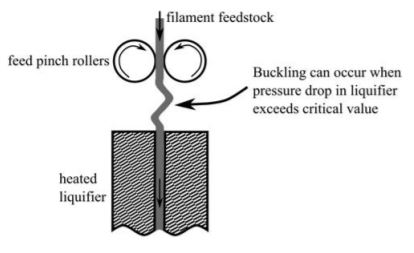
\includegraphics[width=\textwidth]{filamentBucklingReview}
  \end{minipage}
  \hfill
  \begin{minipage}[b]{0.45\textwidth}
    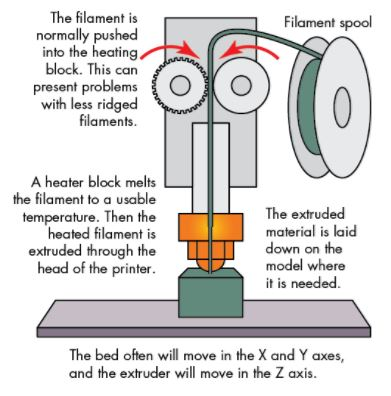
\includegraphics[width=\textwidth]{PinchRollerMachineDesign}
  \end{minipage}
  \\[5pt]
  \begin{minipage}[t]{0.45\textwidth}
    \caption{Illustration of filament buckling \cite{FDMReview}}
  \end{minipage}
  \hfill
  \begin{minipage}[t]{0.45\textwidth}
    \caption{Common machine setup with pinch roller, \cite{MachineDesign}}
  \end{minipage}
\end{figure}

\subsubsection{Pinch-roller}
With pinch roller, material is in form a plastic \textbf{wire}. The wire is \textbf{pinched between two wheels}, with one wheel being smooth and other wheel having grooved of just very rough surface. As the wire is gripped between these wheels, when they rotate, the small gear grips into the wire and pushes it downwards. Principle of operation can be seen in fig. 6.2.

	Since the polymer is not very strong material, there is a force limit. When this force of extrusion is exceeded, the wheels can't push the material - they will loose the grip and tear the surface of the wire instead of pushing it downwards. Also, filament buckling between nozzle entrance and rollers can occur if pressure drop is too high (fig. 6.2).  This setup is used with all low-cost printers, since it is more appropriate for small scales and also is cheaper.
\subsubsection{Screw-feeder}
For larger-scale machines, screw-feeder system would be suitable. This system is also utilized within injection molding machines, where plastic pellets are fed and transported likewise. Screw-feeder has a few advantages over the pinch-roller. First, not only does it transport the material, it also heats the material, lowering required heat source power to reach desired temperature. Second, for larger-scale machines it makes more sense to feed plastic pellets into the machine, instead of a thick wire. Many plastic materials today can be purchased in form of such pellets. Having said the theory, in 2014 there were probably no commercially available FDM printers utilizing screw-feed. \cite[p. 193]{FDMReview}

\section{Available materials}
The range of available materials for FDM use is limited to certain types. As was mentioned in previous section, with the two distinct methods of deposition processes, we have to use either polymer materials in case of heat melting (amorphous polymers are preferred over crystalline polymers), or very specific liquid material designed for this purpose to solidify quickly.

	It should also be mentioned, that the second type of material will require more careful handling. FOr example, in the presence of air it might prematurely solidify, therefore sealed chamber and other additional equipment will be required. That is one of the reasons, why most FDM printers utilize the first type of material, i.e. polymer materials - they are generally speaking easier to process.
	
	To mention some commonly used materials, widely used material is ABS (acrylonitrile butadiene styrene). Also, PLA (Polylactid acid) is material, that is bio-degradable and often used. From other materials, there is Nylon, PET (Polyethylene terephthalate) and others. Also there are materials, that consists of polymer, but are filled with particles of different material such as kevlar, bronze or wood, that might used  for their visual or other preferable properties.
\begin{figure}[h]
	\centering
	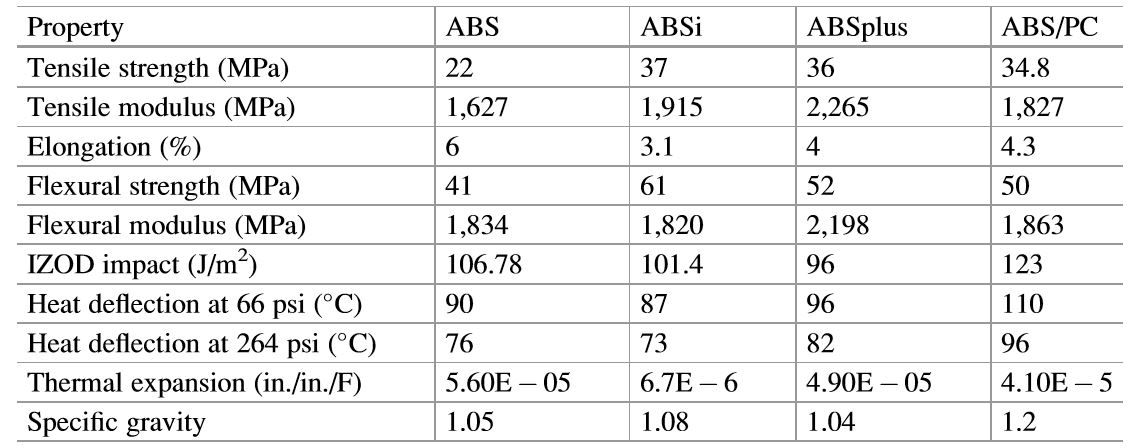
\includegraphics[scale=0.7]{datasheetFDM}
	\caption{Datasheet of some comercially available materials from Stratasys, \cite[p. 163]{AMT}}
\end{figure}
	In last decade, also because of mentioned boom of FDM devices, we experienced growth of supply and demand of suitable materials. Such materials, some of which were developed primarily for purpose of FDM printing, are available with their price ranging from 20EUR (common materials like ABS, PLA) up to several hundreds EUR for 1kg. They can have very wide range of properties, from flexibility, strength, brittleness, resistance to degradation or visual properties.
	
	Regarding flexibility and brittleness, materials can be very stiff having high Youngs modulus and virtually will undergo no elongation, or very flexible as some known polymers that can elongate up to several time of it's original part length. Regarding strength, the range of common polymers is approx 1 order of magnitude smaller compared to metals, that is in range of tens of MPa (Rarely more than 100MPa).

\textbf{We have to be careful when we are generalizing material properties to the final printed part}. When the material is heated and deposited, compared to raw unprocessed material, it can change it's properties significantly - not only can it loose flexibility and become less strong, but for other reasons, we can't also avoid imperfections in the printed part, like small cavities, overlapping difficulties (fig. 6.6) and unisotrophy. For example, when printing part with FDM, in the direction perpendicular to the build platform (direction of following layers), part can withstand less that 1/2 of the original strength before layers separate from each other.

\section{FDM process variations}
Some type variations were already mentioned, such as pinch-roller or screw feed mechanism to push and extrude material through the nozzle.

	When extruding the material, \textbf{not absolute but relative motion} of nozzle and the build platform is controlled. That means that when building a part, there are two options - either the build platform is steady and the nozzle moves around, or nozzle is steady and the build platform moves around. Hence, from construction point of view, we can group FDM machines based on if the nozzle moves, or if the nozzle is a stationary part of the frame and only the build platform moves.
	
	When talking about construction of low-end FDM printers, there is also number of different configurations and various concepts, like deltapod configuration, polar type (having circular rotating build platform) and others. These types with different kinematics can be seen in fig. 6.4, 6.5 and 6.6.

\begin{figure}[h]
  \centering
  \begin{minipage}[b]{0.3\textwidth}
    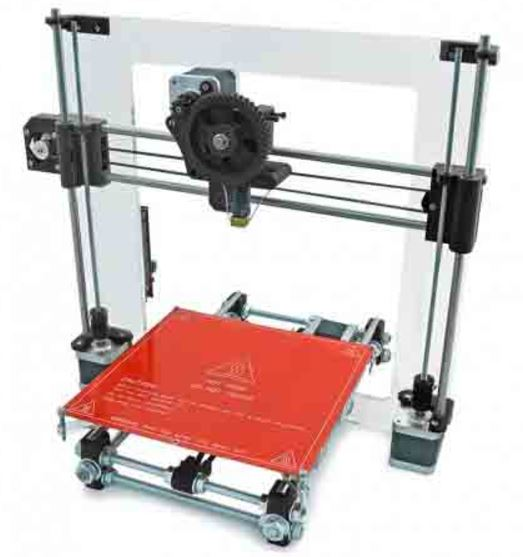
\includegraphics[width=\textwidth]{cartesianPrinter}
  \end{minipage}
  \hfill
  \begin{minipage}[b]{0.3\textwidth}
    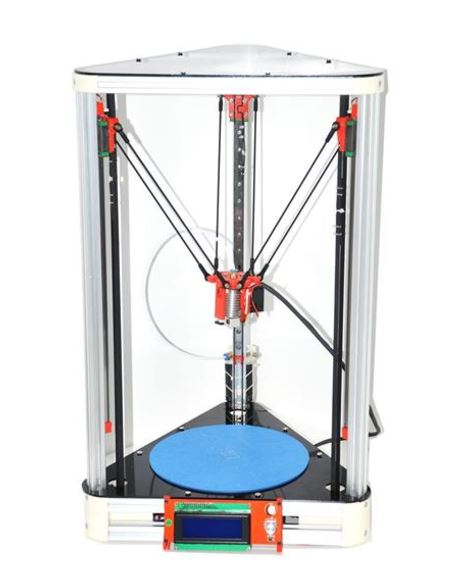
\includegraphics[width=\textwidth]{deltaPrinter}
  \end{minipage}
  \hfill
  \begin{minipage}[b]{0.3\textwidth}
    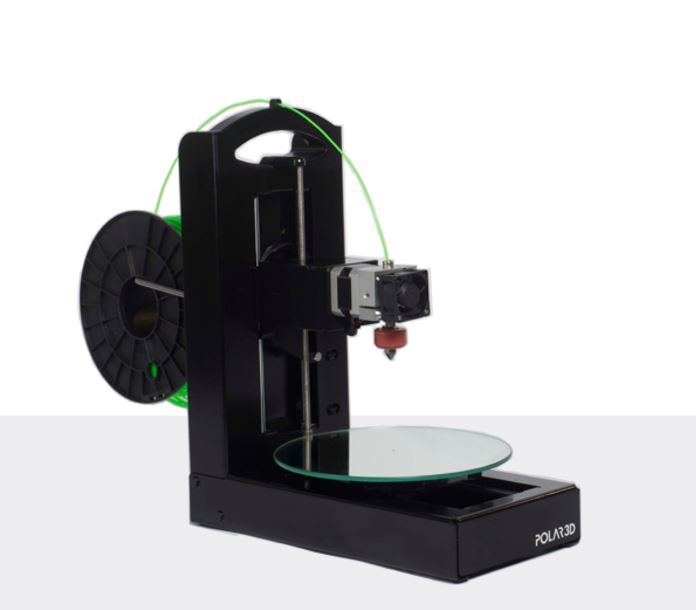
\includegraphics[width=\textwidth]{polarPrinter}
  \end{minipage}
  \\[5pt]
  
  \begin{minipage}[t]{0.3\textwidth}
    \caption{Typical 3-axis cartesian printer}
  \end{minipage}
  \hfill
  \begin{minipage}[t]{0.3\textwidth}
    \caption{Delta FDM printer configuration}
  \end{minipage}
  \hfill
  \begin{minipage}[t]{0.3\textwidth}
    \caption{Rarely used polar configuration, preferable for its high rigidity}
  \end{minipage}
  
\end{figure}
	For high-end and more expensive machines, there are number of additional options and features, usually not utilized by cheap low-end machines. Such features include \textbf{heated chamber} to minimize heat stresses and undesired effects like warping, shrinkage or separation from build platform. Other features might be equipment of various sensors, for example sensor for automatic calibration of the machine (although today already some low-end FDM printers are equipped with such). Also, with low-cost printers utilizing resistor and joule heat to melt the material, other-forms of heating for large-scale machines are possible.

\section{Problematics}
Here, only some of all possible issues are listed, that either follow from the technological principle (hence are unavoidable) or are caused by machine imperfections and can be avoided somehow.
\subsubsection{Accuracy issues}
The main reason of accuracy problem is given diameter of the nozzle, which is finite and can't be changed. For example, let's say we have nozzle exit diameter of 0.4mm. The user is than simply prevented from creating and printing features smaller that 0.4 like sharp chamfers or corners - there is no way of extruding features 0.3mm or smaller.

	Other problem for pinch-roller mechanism and feeding is following - there is a limit speed or material extrusion, given by heating material limitation. Taking example of ordinary low-end FDM printer setup, when the wire with room temperature is fed to the machine, it has to be heated to melting temperature. However, it  also can't exceed some temperature, at which degradation of the material would occur. With given temperature by which wire is heated, we have to remember that the \textbf{wire is heated from the outside}. Still, the whole wire has to melt before being extruded. If the wire was fed too fast to the printer, the outside of the wire would reach sufficient temperature, while the inside of the wire would still be solid, because not enough heat have been conducted to the inside of the wire. When the wire is not sufficiently molten, the nozzle can get clogged, but mainly the flow of material exiting the nozzle will be uneven and unsteady, easily interrupting and ruining the whole printing process.
	
\begin{wrapfigure}{r}{0.6\textwidth}
 	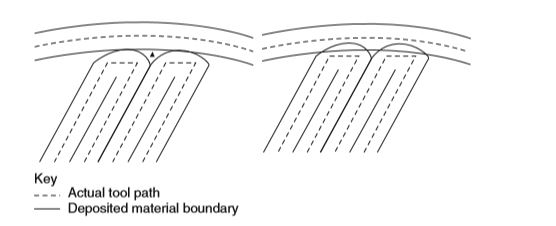
\includegraphics[width=0.6\textwidth]{depositionIllustration}
	\caption{Illustration of trajectory of material deposition trajectory and overlapping, \cite[p. 159]{AMT}}
\end{wrapfigure}
	Next issue is generally problem of support structures for FDM. When printing overhanging features of bridging long distances, need for support structures is present to support the extruded material that doesn't cool enough immediately right after extrusion, and \textbf{can't support it's own weight}. The support structures to hold the printed part in shape, can be printed of the same or different material. If they are printed of the same material, i.e. support structures and the printed part are printed as a single piece, they have to be removed manually after the print. If different material is chosen for support structures, it can be removed usually chemically (i.e. dissolving in water) or manually, which is easier and it leaves us with our final printed part. However, printer with 2 nozzles, one for the basic material and one for support structures material, is needed.
	
	Definitely not all possible problematic of FDM priters were listed. Apart from those mentioned, problems with used software and all related digital part processing - handling of model data, slicing the model and generating the nozzle trajectory can occur. Also, nozzle clogging used to be very common phenomena, which caused troubles to many users.

\section{Conclusion}
\begin{itemize}
\pro \textbf{Price}\\
FDM technology is the cheapest one, making it number one either for home users or small companies or start-ups to help them with product development. Available materials are also very cheap, compared to SLA resins or PBF powders.

\pro \textbf{Ease of use}\\
It might not be found important, but all machines eventually break sometimes. FDM machines are usually relatively easy to clean, maintain and operate.
\\[10pt]



\con \textbf{Speed}\\
FDM is generally slower than many other machines, since it deposits material from single point (nozzle tip), while many other technologies can cure or deposit material simultaneously in multiple places.

\con \textbf{Support structures}\\
With FDM, support structures has to be built to print overhangs or bridging long distances. However, using water-soluble material can make removing support structures very easy.

\con \textbf{Materials}\\
Even though scale of materials is still getting bigger, with FDM one is limited to polymer materials, which can be found of too little strength for functional prototypes or stressed parts.

\con \textbf{Accuracy, surface finish}\\
Compared to other technologies, parts can be relatively less accurate. Sharp edges are impossible to produce due to finite nozzle diameter. Surface quality is low, and especially in the direction of vertical Z axis the surface roughness is poor. For visualization purposes, parts usually require some post-processing.
\end{itemize}

\chapter{Material Jetting}

Printing is an ordinary task, that is part of our daily lives. Various types of desktop printers, such as laser, ink-jet or thermal printers, are commercially available today. However, it was the ink-jet technology, that mostly influenced the development of Material jetting technology (MJ). Even though ink-jet printers and Material jetting machines have different architecture, they share some essential principles of operation. We can say, that by taking the ink-jet 2D printing technology and adding a 3rd dimension, it gave birth to MJ.

\section{Basic operation principles}
Typical machine setup (fig. 7.1). With MJ, all the material - the part structural material and the support material - is dispensed through nozzles from the print head. Material is in liquid state while jetting, and solidifies during or shortly after deposition.  As the print head moves, layer-by-layer small droplets of material are deposited, creating shapes of cross-sections, much like an ordinary 2D desktop printer. After layer is deposited and cured, the build platform is lowered (or print head lifted) by layer thickness, cured layer is optionally smoothed by blade and next layer is deposited and cured. By repeating the process, finished part is obtained.
\begin{figure}[b!]
	\centering
	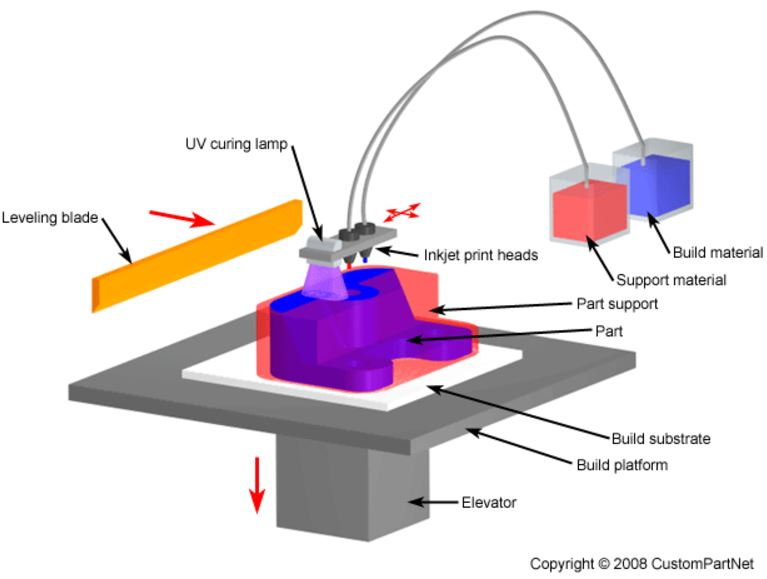
\includegraphics[scale=0.8]{MJmachine}
	\caption{Common MJ machine setup \cite{custompart}}
\end{figure}

\section{Materials for Material jetting}
The material has to exhibit many specific properties to be utilized by MJ. Apart from other requirements, material has to be liquid during deposition able to be jetted, since it has to flow through print nozzles. However, after deposition, it has to solidify very quickly to remain in shape.

\subsection{Material viscosity}
Because of small diameters of nozzle tips (ranging in tens to hundreds $um$), material has to exhibit low-enough viscosity, not to require too high pressure for jetting. Although required pressure is dependent on nozzle diameter and length, for common setups the viscosity shouldn't exceed 40 mPa.s. \cite[p. 176]{AMT}.

	If material with higher viscosity is jetted, either some special system for jetting high viscosity fluids must be used, or the viscosity has to be lowered by some means. For many materials, viscosity drops with higher temperatures, which is the easiest way for lowering viscosity. Use of solvents too is possible \cite{MJ}. Also, shear-thinning effect can occur, reducing required pressure for jetting.

\subsection{Material types}
	Even though polymers today cover the biggest portion of commercial MJ materials, metal or ceramic printing have been performed. Prior to using polymers, MJ depended on wax-based materials.

\subsubsection{Metals and ceramics}
	Metals and ceramics were facilitated only by research groups. Metals were primarily used to fabricate electronic parts, such as PCB, traces and solders \cite{MJmetals}. However, printing metals due to their high melting points often leads to damaging of the print nozzles and surrounding equipment.
	
	Ceramic materials were printed using ceramic suspension, where a ceramic (zirconia powder / alumina particles) are mixed with a solvent. The solvent acts as a binder to hold ceramic material together. After the build process, part must be sintered at high temperatures characteristic to ceramic material to achieve parts of high densities and low porosity.

\subsubsection{Polymers / waxes}
	As of polymer materials, mostly photopolymers are used, same as with SLA. Photopolymers are suitable, since they can be deposited, and subsequently cured with UV light, causing solidification. Such deposition and solidification process can be controlled relatively easily. For easier handling and different material properties, photopolymers partially replaced wax-based materials used before. Such waxy materials, solid at room temperature, were cured simply by beating to temperatures around 100C and subsequent cooling. When heated, wax partially melted and viscosity dropped enough to enable jetting.
	
\section{Process parameters and related problematic}
There are many MJ-specific technical challenges, including droplet formation, deposition process parameters, droplet flight trajectory prediction and others. From all technical challenges, only the most important ones will be addressed.

\subsection{Nozzle-related problems}
When building part with MJ, very high nozzle density within the print head is desired. In other words, more nozzles fitted as close to each other as possible will result in higher part accuracy and smaller features. However, nozzles can't be fitted too close to each other, since pressure field from one nozzle would affect that of adjacent nozzle. Result of such construction problem is compromise between smallest possible feature size, nozzle spacing and construction possibilities.

	Next nozzle-related issue is nozzle clogging. Smaller nozzles require greater pressure difference to form a droplet, but are also more prone to clogging. That might happen, if for example particles in a suspension are too big and block the nozzle, or material solidifies prematurely before nozzle exit. Regular nozzle-cleaning process might be performed during printing.

\subsection{Material solidification}
Material, liquid during deposition, has to become solid shortly after nozzle exit. Depending on the material used, different means of solidification might happen. First, when using a wax-based material, it is heated for deposition and solidifies after due to lowering it's temperature. Second, with cases of i.e. ceramic suspensions, material might solidify due to partial evaporation of liquid from the solution. Third, material can solidify due to chemical reaction, which is case of  mentioned photopolymer curing.

\subsection{Droplet formation}
The problem of viscosity - nozzle diameter relation was already introduced. When a material is pushed through the nozzle, droplets have to be formed. Droplets can be deposited in two distinct ways.
\subsubsection{Continuous deposition}
With continuous deposition, continuous steady stream of droplets is generated from the nozzle by applying pressure to the fluid. In order to control the deposition, some droplets are to be deposited and other droplets have to be separated and discarded before they hit the substrate.

	This is done by charging the droplets of liquid. After leaving the nozzle, before the droplets hit the substrate, they pass through a region of deflector. Deflector can quickly change electric field in the region, thus reacting with charged droplets and controlling their flight-path by electrostatic force. When the droplet is to be deposited, it can pass straight through a deflection field, but when a droplet should not be deposited, it is deflected into a container instead of onto the substrate. Continuous deposition process is able to generate droplets with frequencies of several kHz. However, disadvantage of this approach is that discarded droplets can't be re-used easily, material has to be able to carry a charge, and real-time controlling the deflection field also presents a technical challenge.

\begin{figure}[h!]
	\centering
	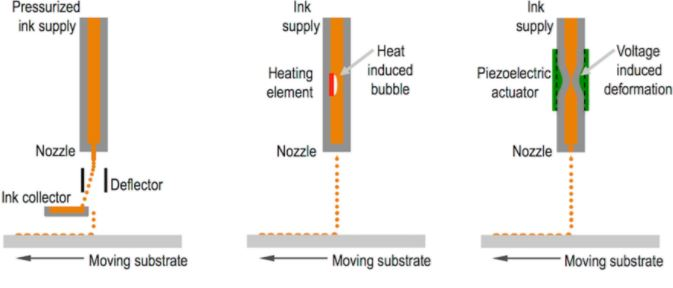
\includegraphics[scale=1]{ContinuousDOD}
	\caption{Continuous and thermal / piezoelectric drop-on-demand deposition \cite{InkjetPrinting}}
\end{figure}

\subsubsection{Droplet on demand}
Droplet on demand (DOD) means that discrete single droplets are generated and deposited only when desired, compared to continuous stream of droplets and disposing unwanted droplets. To generate a single droplet, a pressure pulse is required. To generate a pressure pulse, either thermal or piezoelectric actuator might be used (fig. 7.2).

	Thermal actuator consists of a resistor located inside the fluid reservoir. When heated, a bubble forms, expands and forces a droplet out of the nozzle. The piezoelectric actuator is based on deformation of material when exposed to electric current. With current pulse, the piezoelectric actuator deforms, pressurizing the liquid and forcing a droplet to form.

	While other means of droplet formation exist, they are not commercially utilized by AM and remain a task for researchers.

\subsection{Droplet flight}
When droplet is generated, it is dropped from the tip of the nozzle and falls onto the substrate. The flight distance - distance between nozzle tip and substrate - is usually in range of units of $mm$. It has to be taken into account, that droplet size, shape and impact speed (when hitting the substrate) are important parameters affecting the build quality. For example, too high impact velocities results in droplet splashing, while too low impact speed leads to non uniform and inconsistent material binding. Also, droplet size and shape is important to properly calculate the time of flight from the nozzle tip to the substrate, so that precision of part is ensured.

\section{Conclusion}
\begin{itemize}
\pro \textbf{Cost}\\
Lower cost, relative to other AM technologies (but still costly in absolute terms), is given primarily by using standard components, such as drives, print heads or nozzles. Such components are standard thanks to widespread desktop printing industry. MJ can utilize such components, eliminating need of expensive special equipment such as lasers etc. Material costs however also has to be taken into account, since such materials can be very expensive.

\pro \textbf{Part quality}\\
The overall quality of MJ-printed parts is generally considered very good among AM technologies, with good part accuracy (limited by possible photopolymer shrinkage during polymerization) and surface finish.

\pro \textbf{Print speed}\\
Due to high density of nozzles and line-wise material deposition, printing process is significantly faster compared to other processes, where only single point of current layer can be cured simultaneously (FDM, PBF, SLA, SLS, DED processes). As the build volume gets bigger, lower print times of MJ get more apparent, being possibly more than order of magnitude lower compared i.e. to FDM.

\pro \textbf{Colorful printing}\\
As of today, it is one of the few technologies, that can relatively easily print objects of multiple colors. With MJ, it is done by jetting colorful liquid material from different nozzles or by using additional print head.
\\[10pt]

\con \textbf{Materials available}\\
The range of available materials for commercial use is still limited to photopolymers and wax-based materials, making MJ unsuitable for functional parts production.
\end{itemize}

\chapter{Binder jetting}
Binder jetting (BJ) is a unique AM technology, developed at MIT in 1990s. It is somewhat a combination of PBF and MJ, since it utilizes components, used by these two technologies. 

\begin{figure}[h]
	\centering
	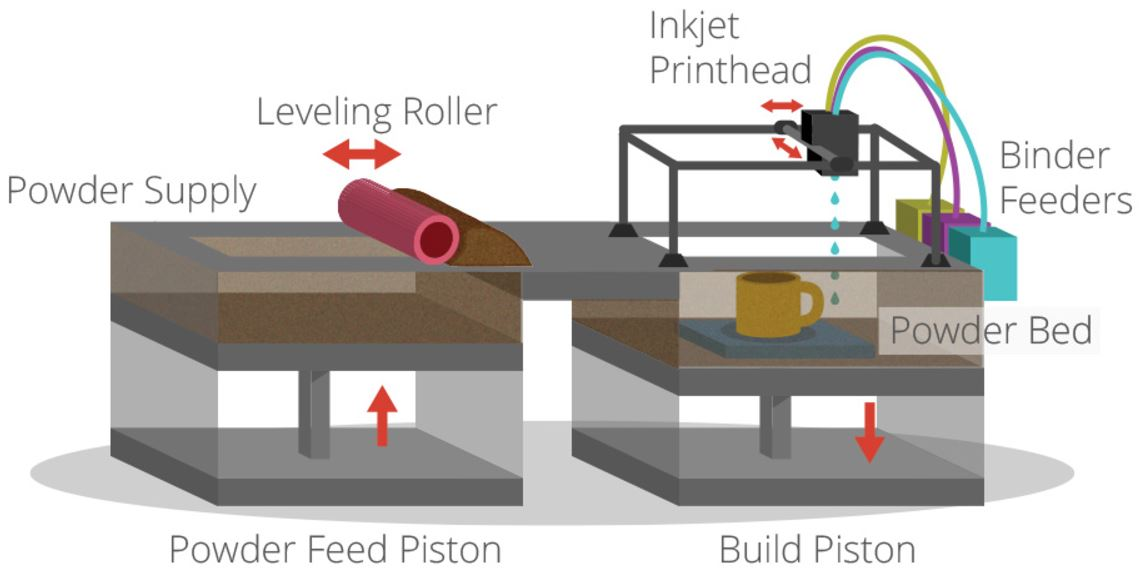
\includegraphics[scale=0.7]{BJthreeding}
	\caption{Schematics of a basic BJ machine, \cite{threeding}}
\end{figure}

\section{Basic operation principle}
Common setup is in the fig. 8.1. The machine works by jetting a binder onto a powder. The used spreading mechanism for powder can be the same as with PBF processes. When a layer of powder is spread and leveled, a binder is jetted onto the powder to form a cross-section shape. After jetting the binder, build platform is lowered by one layer thickness, next layer of powder is spread and the process is repeated until a final part is formed. In contrast with PBF using lasers or electron beam, to bind powder BJ is using print heads like MJ. After completion, part is removed from the powder, cleaned by pressurized air and possibly post-processed and infiltrated to lower part porosity improve mechanical properties.

	Same as with PBF, the loose powder supports upper layers, eliminating need for support structures. Since majority of the material is deposited by spreading mechanism and only low portion is deposited from print head, the whole process can be very fast. The unused loose powder can be recycled straight-away, compared to PBF where powder is affected by heat. Benefit of BJ is that since the building process doesn't involve any heat source, issues of thermal stresses and related shrinkage and warping are not present. Last but not least, thanks to machine architecture and required components, from construction point of view BJ is a technology that can be easily (relative, compared to others AM technologies) scaled, meaning a machine such as Voxeljet VX4000 capable of producing parts of size 4000x2000x1000mm \cite{voxeljet}.

\section{Materials}
Since no heat exposure of powder is present, machine can utilize wide range of materials such as polymers, metals or sand. From other materials, use of ceramic powder with BJ was subjected to research and also plaster can be used \cite[p. 208]{AMT} \cite{ZCorp}. Due to the BJ nature and usable materials, the casting industry is one of the main targets of this technology, particularly for manufacturing sand molds, cores or investment casting patterns.
	
	Apart from choice of structural powder, it is equally important that appropriate structural powder - binder combination is used. For example, plaster material is to be used with water-based binder, where metals usually utilize polymer binder. Wax-based binders are used for production of investment casting patterns with use of suitable polymer, that should exhibit good burn-out properties. On the other hand, foundry sand with appropriate binder are used to produce casting molds and cores.

\section{Process specifications and variations}
Even though not many companies licensed the patent for BJ, there are number differences among such machines and approach differences.

	From those that doesn't require substantial description, optional printing of binder and colorant that enables colorful printing can be mentioned. Also, it should be noted that while machine of different sizes share the same concept, their architecture might be significantly different, because e.g. small machines include small containers for powder that can be manipulated hand-held, while large machines with build volumes of several cubic meters use conveyors. Also, with bigger machines, too low precision with same equipment would be achieved during printing, requiring different components and setup.
	
	Now let's mention some other process characteristics and variations.	

\begin{figure}[h]
	\centering
	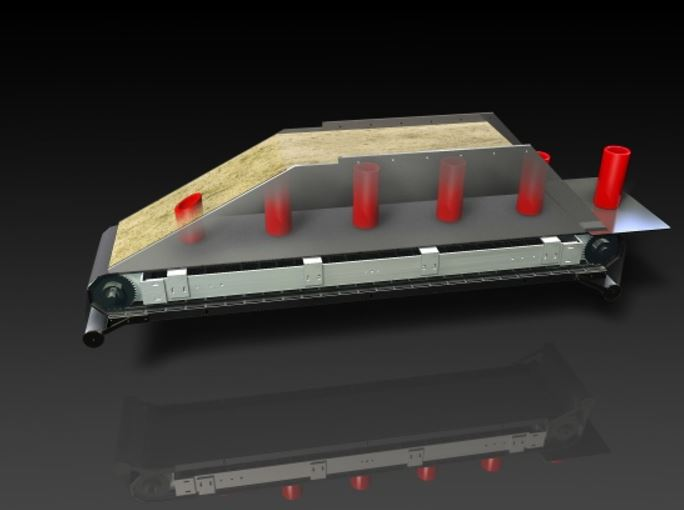
\includegraphics[scale=0.8]{3ders}
	\caption{Voxeljet continuous printing on an inclined plane \cite{3ders}}
\end{figure}

\subsection{Post-processing and infiltration}
As was mentioned, material and binder selection can lead to production of a part with high porosity, and infiltration might be required. Still, prior to infiltration, when printing a part of metal powder with polymer binder, oven curing is required.

	During the oven curing, binder is burned off and metal particles are partially sintered together to improve strength of the part to withstand further manipulation.
	
	Regarding infiltration, ExOne claims production of stainless steel parts infiltrated with bronze at temperatures over 1100$^{\circ}$C, achieving 60\% stainless steel and 40\% bronze part with yield strength of 234 MPa. Another example of bronze infiltration is mentioned in \cite{xometry}.


\subsection{Continuous printing}
Voxeljet utilized a mechanism, that enables printing parts of virtually unlimited length. This is done by depositing powder and binder on an inclined plane, instead of stacking layers horizontally on top of each other. When a current inclined layer is cured, the build platform (here a conveyor) moves sideways and following layer is deposited, as seen in fig. 8.2.

\section{Conclusion}
\begin{itemize}

\pro \textbf{Speed}\\
Since majority of the material is spread via spreading mechanism, the process is very fast compared to other technologies, which is more important with large-scale machines. However, necessary post-processing operations can add to this time, reducing time advantage.

\pro \textbf{Cost}\\
Since BJ shares some specifications with MJ, it also shares utilizing desktop-printing components, reducing price of some key components and the overall cost. The final price still depends on the machine type, used material and size, with small machines costing over 10 000 USD, while the largest Voxeljet priced at almost 2 mil. USD.

\pro \textbf{No heat}\\
Since no lasers or other heat sources are utilized, the part doesn't encounter heat processing, preventing from thermal strains and enabling easy loose powder recycling. Heat processing still might be required for metal parts to burn off the binder and sinter them prior to infiltration.

\pro \textbf{Size capabilities}\\
The size, achievable with BJ machines, is immense, and virtually unattainable for e.g. SLA or FDM because the printing process would be too slow. With one exception of one PBF EB and one FDM machine bigger than VX4000, only comparable technologies to compete with BJ in terms of size are DED or "FDM-like" printers, that utilize similar principle and machine architecture but are many times bigger and deposit concrete to build houses \cite{BigPrinters}.
\\[10pt]

\con \textbf{Accuracy}\\
Even though no warping or shrinkage due to heat is present, the accuracy and surface finishes of final parts are poor compared to other  technologies, given by the fact that the raw powder isn't processed, creating a rough texture.

\con \textbf{Materials, part properties}\\
There is a limited range of commercially available materials, and mechanical properties of final parts are generally worse than e.g. PBF - because no melting or sintering is happening, final part strength is mainly given by the binder agent that is often lower than the structural material strength.

\con \textbf{Post-processing}\\
Post-processing is almost inevitable for metal parts, increasing the time and cost required to produce a single part.
\end{itemize}

\chapter{Sheet Lamination}
Sheet lamination process was first commercialized in 1990s. It works by stacking layers of thin sheet material, that are cut to shapes of cross-sections, stacked on top of each other and bonded, resulting in a final part. The basic idea is simple, enabling the process to be fairly quick. Almost any sheet material, that can be bonded together by some means, can be used, and the choice of used material is closely related to the binding method.

\section{Build process and variations}
The build process starts with raw sheet material. During each step, a sheet is cut to desired shape and bonded to previous layer.

\begin{figure}[h!]
  \centering
  \begin{minipage}[b]{0.45\textwidth}
    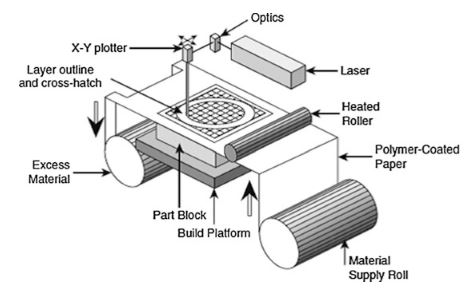
\includegraphics[width=\textwidth]{SL1}
  \end{minipage}
  \hfill
  \begin{minipage}[b]{0.45\textwidth}
    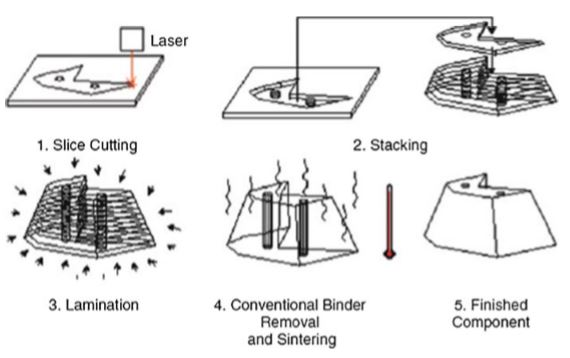
\includegraphics[width=\textwidth]{SL2}
  \end{minipage}
  \\[5pt]
  \begin{minipage}[t]{0.45\textwidth}
    \caption{Bonding, followed by shaping, \cite[p. 220]{AMT}}
  \end{minipage}
  \hfill
  \begin{minipage}[t]{0.45\textwidth}
    \caption{Shaped layers, stacked together, \cite[p. 223]{AMT}}
  \end{minipage}
\end{figure}

	There are two options of layer stacking and bonding - either the current layer is first bonded to previous layer and then cut to shape, or first cut to shape and then bonded to previous layer. Both methods, illustrated in fig 9.1 and 9.2, have their specifics.
	
	When the layer is first bonded and then shaped, the material outside of cross-sectional region is cut to small pieces for easier removal, and remains in place until mechanically removed after the build, so it can serve as support material for overhanging features. However, internal cavities are impossible to create, since excess material can't be removed. Many materials can be used, and material feedstock can be handled easily, so the overall machine architecture is simpler.
	
	The process when material is first cut to shape and then bonded requires more difficult material handling, resulting in higher machine costs. However, the benefit of such method is that there is no risk of cutting into previous layers, since layer is not cut on top of other layers. Also, internal cavities can be created, because the loose excess material is not deposited.
	
	Regarding the cutting process, commonly a laser or a mechanical knife is used for cutting. When layers are first bonded and then cut, the cutting tool has to be very precisely configured to cut only to the depth of one layer, which can be very difficult. Combination of SL machine with CNC machine, using milling mechanism to cut and shape single or already stacked layers, is possible and can improve the overall quality and surface smoothness.

\section{Materials}
Since there are many ways how sheets can be bonded together, virtually any sheet material can be used. Most common materials, whose use was already commercialized, are paper and metal.

	Paper was the first material used for SL, since it can be bonded together by relatively ordinary glue, enabling easy binding process. After gluing and stacking, resultant part is fairly strong. Today, SL machines using ordinary office papers are available, whose benefit is very cheap and easily available feedstock \cite{mcor}.

	For metals, cutting process can be the same as with paper, but different binding processes are utilized (mentioned in following section). Aluminum and steel foils are used, with the thickness varying usually around cca. 0.2 mm.
	
	Other materials for SL include e.g. ceramics and polymers. Ceramic tiles can be formed by mentioned means, same as with polymers. Commercially succesfull machine of Solidimension utilized PVC sheets \cite{cubic}. When considering production of a bigger parts, cutting big pieces of foam by hot wire and stacking them on top of each other is an old sculpting method that can also be considered as SL.

\section{Binding processes}
Sheets of default material can be bonded by various means, depending on the material properties. Some methods are suitable for metals, other for paper or ceramics.

\subsection{Thermal bonding}
Thermal bonding is activated by heat source, that elevates temperatures so that bonding can occur. One way of utilizing thermal bonding is using sheets of material, coated with another material with lower melting point. When pressed and heated to certain temperature, coating material melts and during solidification binds adjacent layers, while structural material remains solid. Another example of heat-actuated bonding can be solid-state diffusion, happening at elevated temperatures. Such thermal-caused bonds typically exhibit very good strength.

\subsection{Clamping}
Clamping is an easy way of binding. It is simple mechanical method, when stacked layers are pressed together by some means and held together. That approach is generally inexpensive, since it doesn't require any special equipment and is easy to utilize. However, it's major drawback is limitation of a part shape, since clamping force has to be applied perpendicular to layers and part shape has to be adjusted to this condition.

\begin{figure}[h!]
	\centering
	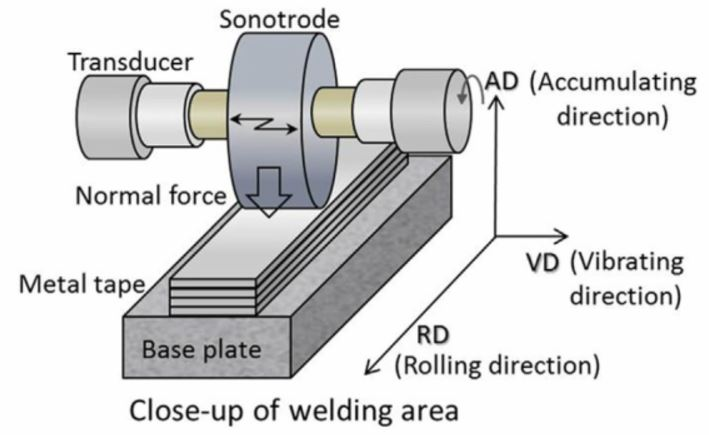
\includegraphics[scale=0.8]{sonotrode}
	\caption{Schematic of ultrasonic metal welding SL machine, \cite{sonotrode}}
\end{figure}

\subsection{Adhesive bonding}
Such bonding is mostly used with paper materials. First SL technology used paper, coated with polymer adhesive. Using glue doesn't require any additional treatment, but can be less strong. When using polymer binding, the binder under the top layer is activated by some mechanism, that moves over the top layer and heats it, so that the heat  activates the binder under the layer and causes joining.

\subsection{Ultrasonic welding}
Ultrasonic welding (UW) is suitable for metal sheets of various thicknesses. However, contradictory to it's name, the means of bonding are not plain simple as welding, but it is much more intricate process. Compared to welding, the temperature during UW doesn't usually go anywhere near melting temperature of the metal, and the overall UW process can be combination of multiple bonding mechanisms including diffusion, melting and forces on atomic scale. There are many parameters during ultrasonic welding to set properly to achieve well welded defect-free regions, making UW hard to master. Still, the UW binding can be of great quality, ensuring necessary proper joining of layers that will maintain strength during higher temperatures or when stressed. However, UW made parts will exhibit great amount of anisotropy that has to be taken into account, when delimiting part's working conditions.

\section{Conclusion}
\begin{itemize}
\pro \textbf{Speed}\\
Because only the outline of the cross-section has to be cured - cut, the process can be much faster compared to processes such as PBF or FDM, where the whole cross-section has to be traced.

\pro \textbf{Cost}\\
Even though more expensive than low-cost FDM machines, the SL machines for small scale products are on the cheap end of AM machines spectrum, with possible cheap paper feedstock material. More expensive machines might use higher-powered lasers or incorporate CNC machining process within the machine, improving the final part accuracy and surface roughness.

\pro \textbf{Materials}\\
Wide range of materials is potentially usable with SL, despite the fact not all materials are commercialized for SL use. In general, SL technology can also be considered quite versatile, producing robust parts and suitable for many industries.
\\[10pt]

\con \textbf{Layer binding}\\
The process of SL faces some technical obstacles, especially regarding joining distinct layers by UW.

\con \textbf{Part complexities}\\
Although with shaping and subsequent cutting internal cavities and similar features can be made, SL is generally not the technology best suited for creating part with such features or complex 3d curved shapes.

\con \textbf{Excess material removal}\\
The excess material, outside of the part cross section, is cut to smaller cubes, but removal of excess material can still be a tedious difficult task, making SL less user-friendly and more time and work consuming.
\end{itemize}

\chapter{Directed energy deposition processes}

Directed energy deposition (DED) is AM technology, that although not literally combine pieces of PBF and FDM technology. With DED, energy source is focused into a small region. When the material is deposited into this focused region, it instantly melts, creating a melt pool. As the heat source moves away, it leaves behind a track of solidified material. To prevent material degradation during high temperatures, a sealed chamber with vacuum or inert gas is used, or shielding gas usage is necessary. Common DED machine setup is in the fig. 10.1.

\begin{figure}[h]
	\centering
	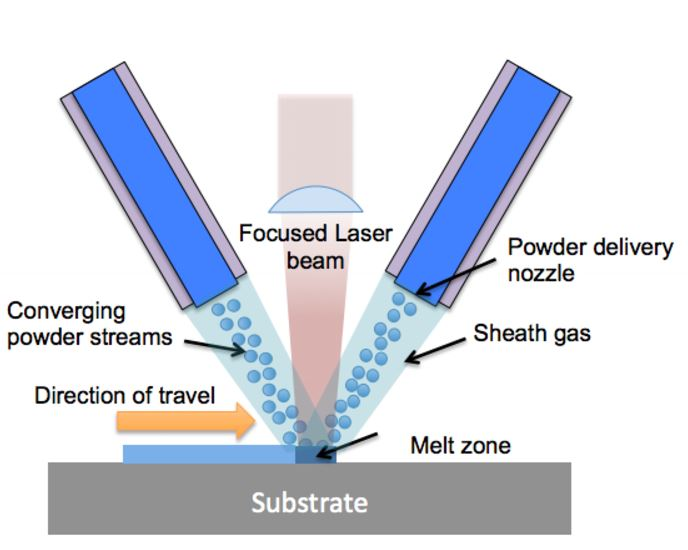
\includegraphics[scale=0.7]{DED3dprinting}
	\caption{Common DED machine setup, using laser and powder feeding, \cite{3dprinting}}
\end{figure}

\section{Materials}

In theory, any material that can melt and solidify more times can be used, same as PBF. However, most of DED machines are made for metal processing.

	Pure ceramics is not easy to process - not all ceramic materials actually can be molten. Furthermore, cracking can easily occur, to which ceramics is more prone than metals.

\subsection{Metal processing}
Whether DED machine uses metal powder of wire, it shares some aspects with PBF. For both technologies, a metal is generally suitable if it's weldability is good. Also, reflective materials or materials with high thermal conductivity, are more difficult to process. Steel, stainless steel, titanium, inconel, CoCrMo or other alloys are used.

	An advantage, shared with PBF, is possibility of achieving unique micro-structure of a part, but with DED the process parameters (and hence final properties and structure) are more versatile and controllable. If high cooling rates are dealt with properly avoiding thermal stresses and shrinkage, it leads to several benefits - having a very small heat affected zone, possibly achieving non-equilibrium phases, uniform structure and very small grain size. By changing the build parameters, user can achieve different properties of the part.

\begin{figure}[b!]
	\centering
	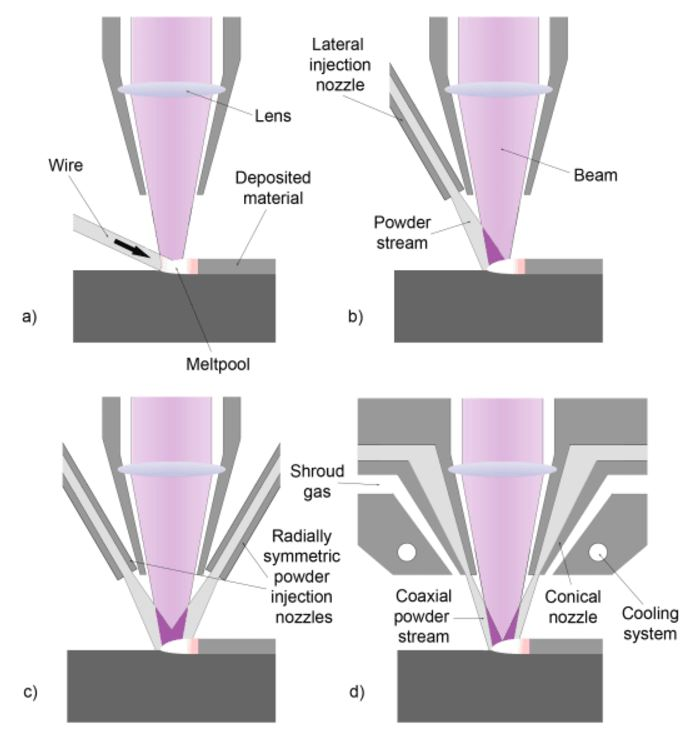
\includegraphics[scale=0.8]{DEDnozzles}
	\caption{Different feeding mechanisms \cite{engineering}}
\end{figure}

\subsection{Material form}
As it follows, material can be fed into the heat source as a wire or in form of powder. Both variants have some benefits and drawbacks.
\subsubsection{Powder feeding}
When powder is sprayed into the beam, not all of the powder is caught, melted and deposited. The material efficiency is therefore not 100\%, although still very high. However, utilizing powder in general tends to be easier compared to wire feeding. To successfully spray the powder from the container where it is held, the power has to be "fluidized" so that the flow is consistent. That is done by ultrasonic vibrating of the container, or bubbling air through the container \cite[p. 251]{AMT}.
\subsubsection{Wire feeding}
Wire feeding is more appropriate for simple part geometries. Paradoxically, the 100\% feedstock efficiency tends to cause problems. For example, when the overlapping of two adjacent tracks of material increases, the excess material is pushed out of the melt pool. All in all, with wire feeding it is hard to achieve and keep part precision, therefore powder feeding is more common approach for commercial DED machines. However, a huge benefit of wire feeding is much higher deposition rate.

\section{Process variations}
Same as with any other technology, there are many differences in approaching various technical challenges of DED processes.


\subsection{Heat source}
DED machines use laser or electron beam as the heat source, that determine material limitations (like conductive materials for EB), that with other related characteristics are also shared with PBF. The heat source parameters, including power or spot size, are strongly related to other parameters such as scanning speed or melt pool size. Both EB and laser operate in the vacuum sealed chamber, possibly with as little as 10ppm oxygen\cite[p. 252]{AMT}. For lasers, an alternative is protection from degradation by supplied shielding inert gas. 
\subsection{Nozzle distribution}
When powder material is used, it travels from the container to the melt pool region through a nozzle. Nozzle shapes and their numbers for powder feeding are another process parameter.
	
	As shown in the fig. 10.2, machine can use either single coaxial nozzle, or one or more single nozzles. With coaxial nozzle, the material is fed to the beam from all sides simultaneously. That results in more uniform structure, but at the expense of component simplicity and therefore cost. When using a single nozzle, the advantage is it's lower cost, but same as with welding, because of preferred feeding direction there will be preferred grain growth direction and other unisotropical effects. This can be avoided by using multiple single nozzles, all of them focused into a single point.

\section{Conclusion}
\begin{itemize}
\pro \textbf{Material properties}
With metal DED, parts can exhibit very fine micro-structure with high strength and other functional properties, due to high cooling rates.

\pro \textbf{Deposition versatility}
Inherently to the process specification, from all AM technologies only DED is capable of not only creating a new part, but of depositing a material onto already existing part. That can be very useful for e.g. depositing a wear-resistant coating and subsequent machining to die-casts of injection molds, or to repair parts by depositing material on worn locations, followed by machining to achieve original dimension and accuracy.

\con \textbf{Speed}
Although dependent on the heat source power, deposition rate is usually very low, ranging in tens of g/min /cite{WireFeed}. Wire feeding mechanism exhibits much higher deposition rate, but is subjected to other technical difficulties.

\con \textbf{Geometric restraints}
Support structures are not easily built. For complex geometries, necessary support structures have to be built and afterwards mechanically removed. Such mechanical removal adds up to the already long build time and overall cost.

\con \textbf{Part quality and accuracy}
Even if the flow of powder is relatively uniform, inherent to the process is very poor part accuracy and surface finish, that can exceed Ra200 \cite{WireFeed}. Still, DED machine can be combined with CNC machinery, creating hybrid additive-subtractive production machine with high precision and accuracy typical for CNCs.
\end{itemize}


\chapter{Tensile strength of parts printed with FDM}
The technology of Fused Deposition Modeling, or Fused Filament Fabrication (FDM/FFF) was described previously. This thesis consists also of practical and experimental section, which is based on FDM. The task was to find, what effect do \textbf{print parameters of FDM}, such as layer thickness, infill amount etc, have on \textbf{strength} of the final part.\\
\section{General properties of FDM prints}
There are multiple reasons why such knowledge is valuable and important. Obvious reasons are, during parts design we always have to be aware of the part production process - different manufacturing procedures may result in different properties of the same part geometry. This is mostly due to anisotropical nature of such processes. When we are talking about FDM, the process is very anisotropical with parts having different properties in X/Z build direction (plane of single layer) and Z direction (vertical direction of build). Probably all kinds of macroscopic properties will show some amount of anisotropy, such as heat conductivity or electric conductivity. This is generally applicable on AM, i.e. plastics used with FDM are bad electricity conductors. For mechanical engineering, however, the crucial property that will vary with changing direction is strength and elongation of the material.\\
\section{FDM and injection molding}
Another important reason for such research is that we should be able to make a direct comparison between strength of part of the same geometry and made of the same material, but produced using different technologies. Particularly useful is the ability to compare parts made with \textbf{injection molding} and \textbf{additive manufacturing}. Both are using polymer materials and processing them by heat. For injection molding, the part will also be somewhat anisotropical, which is caused by the flow direction of the plastic. Compared to FDM however, injection molded parts will be much more isotropical and uniform.\\
The difference here can be of great significance, when we are considering production of functional, i.e. stressed parts. We know that injection molding and AM are on the opposite ends of the spectra of production rate, with molding being extremely productive with high quantities and AM being very slow. Nonetheless, if we find out that only very limited of parts is to made made (ranges of $10^0$ up to $10^3$ pieces), it is rational to think of AM instead of injection molding. On the contrary, AM produced parts due to it's nature will show different strength and elongation. Therefore production technology has to be accounted for before the production itself.
\begin{figure}[b]
\centering
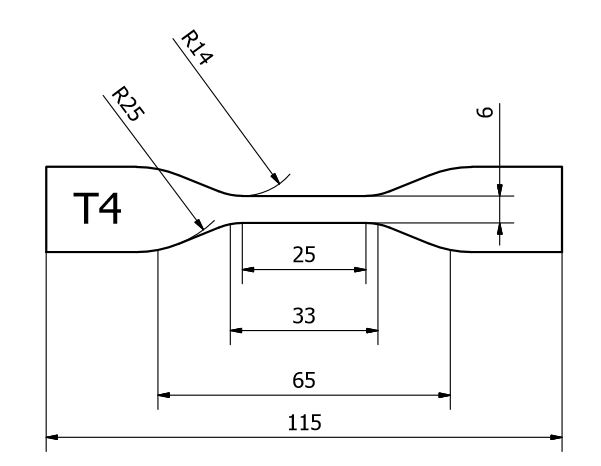
\includegraphics[scale=0.6]{testSpecimenDimensions}
\caption{ASTM D638 - dimensions of test specimen type 4}
\end{figure}
\
\todo[inline]{misto pro nejakz obrazek}
\newpage
\section{Print parameters}
Following parameters were to be examined:
\begin{itemize}
\item \textbf{Layer thickness}\\
	Different thickness of individual layers, range from 0.1 - 0.25 mm
\item \textbf{Infill}\\
	Amount of infill, range from hollow = 0\% up to full = 100\%
\item \textbf{Print temperature}\\
	Different setting of the constant nozzle temperature during extrusion
\item \textbf{Infill raster orientation}\\
	Orientation of rectilinear raster pattern, angle with edges in range of 0$^{\circ}$ - 45$^{\circ}$
\item \textbf{Layer orientation}\\
	Part build on different sides - different orientation of build
\item \textbf{\textit{Default parameters}}\\
Layer thickness 0.1mm\\
Infill 100\%, rectilinear pattern\\
Print temperature 240$^{\circ}$C\\
Infill raster orientation 45$^{\circ}$\\
Layer orientation - parallel to stress direction
\end{itemize}
\bigskip
%
Other print settings and parameters remained constant, and are listed as follows:
\begin{itemize}
\item \textbf{Material}\\
	PETG
\item \textbf{Nozzle diameter}\\
	1.75mm/0.4mm
\item \textbf{Overlap of material}\\
	25\%
\item \textbf{Shell / outside circumference region thickness}\\
	3 shell lines (outside of infill pattern)
\item \textbf{Number of top layers}\\
	12
\item \textbf{Bottom layers}\\
	10
\item \textbf{Build speed}\\
	Perimeters - 25-40mm/s\\
	Infill - 30-60mm/s
\item \textbf{Other}\\
	No raft generated
	No support material / support structures
\end{itemize}
For making test specimen, 3D printer Prusa I3, borrowed from Prusa company (mentioned in acknowledgements) was used. Slicer software used for Gcode generation was Prusa slicer ver. 1.31.6. The test specimen has a shape as in fig. 5.1. The shape is given by the ASTM D638 standard, used for plastic parts made by injection molding or machining. Up to this date there is no other generally accepted standard for 3D printing specimen for tensile strength testing.\\
Material used was PETG, provided by Prusa company - no corresponding datasheet with material properties was available, only recommended print temperature 220-250$^{\circ}$C was listed. For tensile strength testing, deformation rate of 50mm/min and 20mm/min were observed. Standard tensile strength testing machine with grips for plastic specimen was used.\\
After testing two sets of 5 specimen, each with different deformation rate, there was no difference in tensile strength observed between specimen stressed with 20mm/min and 50mm/min rates. It was therefore concluded, that for purposes of this thesis and limited time of tensile strength machine availability, deformation rate 50mm/min will be sufficient.
%
\newpage
\section{Tensile strength testing results}
\textbf{Changing layer thicknesses}\\
\begin{tabular}{|c|c|c|}
\hline 
Layer thickness [mm] & Tensile strength [MPa] & Elongation [\%]\\ 
\hline 
0.10mm & 46.23 $\pm$ 1.59 & 5.48$\pm$0.25\\ 
\hline 
0.15mm & 40.20 $\pm$ 4.60 & 5.38$\pm$0.44\\ 
\hline 
0.20mm & 47.14 $\pm$ 1.57 & 5.80$\pm$0.14\\ 
\hline 
0.25mm & 41.36 $\pm$ 0.77 & 5.55$\pm$0.16\\ 
\hline 
\end{tabular}
\\[20pt]
%
\textbf{Changing rectilinear infill raster orientation}\\
180 = parallel to force direction\\
90 = perpendicular to force direction\\
\begin{tabular}{|c|c|c|}
\hline 
Angle orientation [deg] & Tensile strength [MPa] & Elongation [\%]\\ 
\hline 
45/135 & 46.23 $\pm$ 1.59 & 5.48 $\pm$ 0.25\\ 
\hline 
60/150 & 40.46  $\pm$ 1.46 & 4.86 $\pm$ 0.31\\ 
\hline 
75/165 & 42.33 $\pm$ 1.23 & 4.90 $\pm$ 0.29\\ 
\hline 
90/180 & 43.48 $\pm$ 1.78 & 4.91 $\pm$ 0.38\\ 
\hline 
\end{tabular}
\\[20pt]
%
\textbf{Changing nozzle temperature for printing}\\
\begin{tabular}{|c|c|c|}
\hline 
Nozzle temperature [C] & • Tensile strength [MPa] & Elongation [\%]\\ 
\hline 
220 & 38.77 $\pm$ 3.16 & 5.13 $\pm$ 0.52\\ 
\hline 
230 & 43.73 $\pm$ 0.93 & 5.37 $\pm$ 0.21 \\ 
\hline 
240 & 46.23 $\pm$ 1.59 & 5.48 $\pm$ 0.25 \\ 
\hline 
250 & 43.46 $\pm$ 0.46 & 5.10 $\pm$ 0.21\\ 
\hline 
\end{tabular}
\\[20pt]
%
\textbf{Changing infill percentage}\\
\\pozn. - infill is related to the inside of the print, the outside boundary is always kept solid. As was mentioned in the print parameters section, there were always 10 solid bottom layers, 12 solid top layers, and also circumference is always built solid. Therefore, the amount of material in the cross-section is much more, than only solid model multiplied by infill percentage. In other words, approximately only inner $8mm^2$ are filled with infill, remaining $16mm^2$ of the cross-section are always built solid.\\
\begin{tabular}{|c|c|c|}
\hline 
Infill [\%] & Tensile strength [MPa] & Elongation [\%]\\ 
\hline 
100 & 46.23 $\pm$ 1.59 & 5.48 $\pm$ 0.25\\ 
\hline 
80 & 46.30 $\pm$ 0.82 & 5.46 $\pm$ 0.14\\ 
\hline 
60 & 45.14 $\pm$ 0.92 & 5.62 $\pm$ 0.92\\ 
\hline 
40 & 37.03 $\pm$ 4.39 & 4.46 $\pm$ 0.57\\ 
\hline
20 & 39.38 $\pm$ 6.31 & 4.58 $\pm$ 0.86\\ 
\hline 
\end{tabular}
\\[20pt]
%
\textbf{Layers orientation with respect to force direction}\\
XY - standard, layers in plane parallel to force direction\\
XZ - non-standard, layers perpendicular to force direction, no elongation and lower strength expected
\begin{tabular}{|c|c|c|}
\hline 
layers orientation parallel to plane [\%] & • Tensile strength [MPa] & Elongation [\%]\\ 
\hline 
XY (standard) & 46.23 & 1.59\\ 
\hline 
XZ (vertical build) & IDK & IDK\\ 
\hline
\end{tabular}
\\[30pt]
During performing the tensile strength tests, unexpected behavior of test specimen was observed many times. Also, as can be seen in results table, there are some significant inconsistencies among tested specimen. Compared to usual tensile strength testing results of injection molded test specimen, standard deviation can be very high. Inconsistencies occur not only within a single group of test specimen (specimen printed with the same parameters), but also within a single changing parameter (inconsistent results, uneven illogical changes of strength with changing i.e. layer thickness). Also because many specimen showed different behavior, there was question which specimen should be taken as relevant, and which results should be discarded. Because there is no guide, we took all the data, which include even results of extreme values. This is reflected in higher standard deviation of the final strength value.
%
\begin{figure}[!t]
  \centering
  \begin{minipage}[b]{0.45\textwidth}
    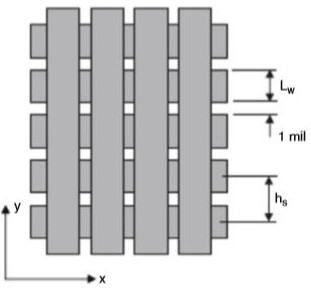
\includegraphics[width=\textwidth]{weave1}
  \end{minipage}
  \hfill
  \begin{minipage}[b]{0.45\textwidth}
    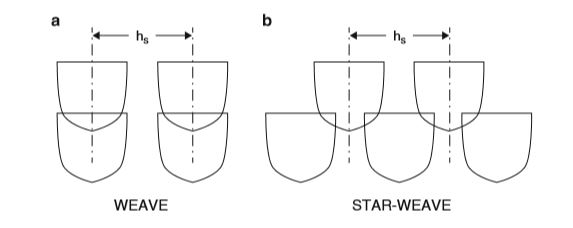
\includegraphics[width=\textwidth]{weave2}
  \end{minipage}
  \\[1pt]
  \begin{minipage}[t]{0.45\textwidth}
    \caption{Test specimen broken outside of narrow region}
  \end{minipage}
  \hfill
  \begin{minipage}[t]{0.45\textwidth}
    \caption{Delamination / separation of part shell from infill part}
  \end{minipage}
  %
  \\[5pt]
  %
 \begin{minipage}[b]{0.45\textwidth}
    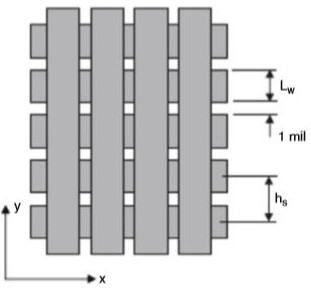
\includegraphics[width=\textwidth]{weave1}
  \end{minipage}
  \hfill
  \begin{minipage}[b]{0.45\textwidth}
    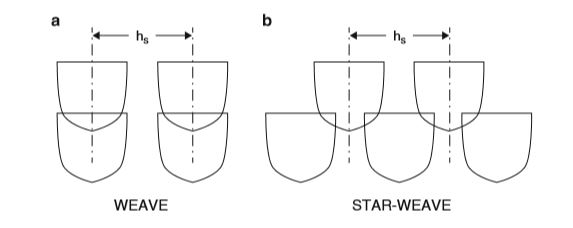
\includegraphics[width=\textwidth]{weave2}
  \end{minipage}
  \\[1pt]
  \begin{minipage}[t]{0.45\textwidth}
    \caption{Illustration of imperfect overlapping and gaps in infill}
  \end{minipage}
  \hfill
  \begin{minipage}[t]{0.45\textwidth}
    \caption{Unusual break line of specimen}
  \end{minipage}
  %
  \\[5pt]
  %
   \begin{minipage}[b]{0.45\textwidth}
    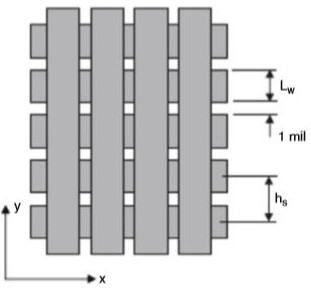
\includegraphics[width=\textwidth]{weave1}
  \end{minipage}
  \hfill
  \begin{minipage}[b]{0.45\textwidth}
    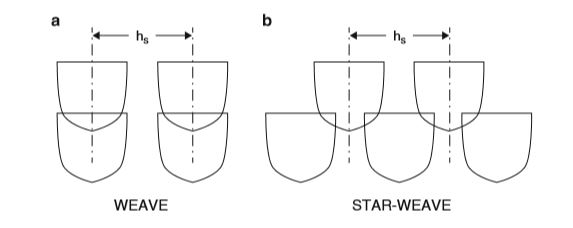
\includegraphics[width=\textwidth]{weave2}
  \end{minipage}
  \\[1pt]
  \begin{minipage}[t]{0.45\textwidth}
    \caption{Elongation of single thread, separated from part during stressing}
  \end{minipage}
  \hfill
  \begin{minipage}[t]{0.45\textwidth}
    \caption{Cross section of broken specimen, showing brittle fracture with little elongation}
  \end{minipage}
  \\[5pt]
\end{figure}
%
\\Other parameters, that were not tested but could have significant effect on strength value, are listed below:
\begin{itemize}%[leftmargin=5]
\item \textbf{Infill pattern}
	It is likely that different infill patterns will show different strength and elongation with the same infill percentage.
\item \textbf{Time since last printer activity}\\
	It might be important, how long the printer was idle and not active.
\item \textbf{Age of material}\\
	Effect of material aging and degradation can also be worth researching.
\item \textbf{Printer quality and software used}\\
	Different printers might be able to print parts of different strengths. Reasons can be those of different printer stiffness (influencing part build consistency), consistency of nozzle temperature (causing inconsistencies in the material flow and build), bad slicer software and generation of unsuitable G-code and others parameters, that are not directly open to the users to manipulate with
\item \textbf{Environment conditions}\\
	Humidity and temperature, in combination with other parameters, might affect the material properties
\end{itemize}
Delamination\\
Break outside of grips\\
otazka jake vzorky vyradit jake nechat, nejake se pretrhly jine se prodluzovaly 3x, nahodny smer praskani - nekonzistentni, striska, vliv tloustky steny
\\Co ma nejvetsi vliv nejsou parametry, ale design, praskani nastava na rozmezi infillu a obvodu, vysledky taky nejsou jednoznacne, nicka opakovatelnost a vysoky rozptyl hodnot pevnosti - odchylka je vetsi nez rozptyl, vliv rychlost deformace
\\Vliv doby stani tiskarny, popsat trhani, ceho jsme si vsimli, jake vzorky vyhodit jake ne, vliv rychlosti deformace, rychlost dle normy, testovani struny a porovnani hodnoty nezpracovaneho materialu
\todo[inline]{ziskat data elongation, a cely prubeh zkousky}
\todo[inline]{Datasheet}

\listoftodos

\begin{thebibliography}{99}
	\bibitem{AMT}
	Gibson, I. \& Rosen, D. \& Stucker, B.,
	2015.
	Additive manufacturing technologies
	2nd ed.
	Springer:
	New York, Heidelberg, Dordrecht
	ISBN 978-1-4939-2112-6
	
	\bibitem{FirstPatent}
	Hull, Charles W.
	Apparatus for production of three-dimensional objects by stereolithography,
	US4575330 A,
	USA,
	8.8.1984
	
	\bibitem{CrumpPatent}
	Crump, Scott. S,
	Apparatus and method for creating three-dimensional objects,
	US5121329 A,
	USA,
	30.10.1989
	
	
	\bibitem{JointReplacement}
	Trebše, R.
	Infected Total Joint Atrhoplasty - The algorithmic Approach,
	2012,
	ISBN: 978-1-4471-2481-8
	
	\bibitem{DentalPrinter}
	ENVISIONTEC,
	[online],
	last revision 13.3.2017,
	<https://envisiontec.com/3d-printers/desktop-3d-printers/vida>
	
	\bibitem{AMOrigins}
	3D PRINTING INDUSTRY,
	[online],
	2017,
	last revision 13.3.2017,
	<https://3dprintingindustry.com/3d-printing-basics-free-beginners-guide/history/>
	
	\bibitem{WoodenFilament}
	MATTER HACKERS,
	[online],
	2017,
	last revision 13.3.2017,
	<https://www.matterhackers.com/store/3d-printer-filament/175mm-wood-filament-light-cherry-0.25-kg>
	
	\bibitem{MachineDesign}
	MACHINE DESIGN,
	[online],
	2017,
	last revision 19.07.2017,
	<http://www.machinedesign.com/manufacturing-equipment/3d-printing-tips-and-tech-get-know-those-acronyms>
	
	\bibitem{unconn}
	UNCONN SLS,
	[online],
	2017,
	last revision 24.07.2017,
	<http://www.engr.uconn.edu/~xchen/sls/>
	
	\bibitem{xometry}
	Xometry
	[online],
	2017,
	last revision 24.07.2017,
	<https://www.xometry.com/metal-binder-jetting>
	
	\bibitem{chinese}
	3D PRINTING LAB
	[online],
	2017,
	last revision 24.07.2017,
	<http://www.3dprintinglab.com.hk/blog/using-powder-based-printing-material-sls-3d-printing>
	
	\bibitem{SLAmaterials}
	Jacobs PF,
	1992,
	Rapid prototyping \& manufacturing,
	fundamentals of stereolitography,
	SME,
	New York
	
	\bibitem{FDMReview}
	Brian N. Turner, Robert Strong, Scott A. Gold,
	2014,
	A review of melt extrusion additive manufacturing processes: I. Process design and modeling,
	Rapid Prototyping Journal, Vol. 20 Issue: 3, pp.192-204,
	https://doi.org/10.1108/RPJ-01-2013-0012
	
	\iffalse
\bibitem{AMT}
	GIBSON, I. \& ROSEN, D. \& STUCKER, B.,
	2015.
	Additive manufacturing technologies
	2nd ed.
	Springer:
	New York, Heidelberg, Dordrecht
	ISBN 978-1-4939-2112-6
		\fi
		
\bibitem{LPS}
	German, R. M.,
	1985,
	Liquid Phase Sintering,
	Springer,
	New York
	ISBN 978-1-4899-3601-1 / ISBN 978-1-4899-3599-1 (eBook)
	DOI: 10.1007/978-1-4899-3599-1

\bibitem{MJ}
	H. Yang, Y. He, C. Tuck, R. Wildman, I. Ashcroft, P. Dickens, R. Hague,
	2013,
	HIGH VISCOSITY JETTING SYSTEM FOR 3D REACTIVE INKJET PRINTING,
	Additive Manufacturing and 3D printing group - University of Nottingham - UK 

\bibitem{MJmetals}
	Liu Q., Orne M.
	2001,
	High precision solder droplet printing technology and the state-of-the=art,
	J matter process technology,
	115:271-283
	
\bibitem{custompart}
	custom part,
	[online],
	2017,
	last rev. 27.7.2017
	<http://www.custompartnet.com/wu/jetted-photopolymer>
	
\bibitem{ZCorp}
	3D molecular design,
	[online],
	2017,
	last rev. 30.07.2017,
	<http://www.3dmoleculardesigns.com/Custom-3D-Print-Molecular-Models/ZCorp-3D-Printer.htm>

\bibitem{AdditiveSubtractive}
	Ambrosi, Adriano and Pumera, Martin,
	3D-printing technologies for electrochemical applications,
	Chem. Soc. Rev. vol. 45 issue 10. p. 2740
	2016,
	The Royal Society of Chemistry,
	doi:10.1039/C5CS00714C,
	http://dx.doi.org/10.1039/C5CS00714C,

\bibitem{threeding}
	threeding,
	[online],
	2017,
	last rev. 29.7.2017
	<https://www.threeding.com/blog/\%E2\%80\%8Bbinder-jetting-3d-printing-technology>
	
\bibitem{voxeljet}
	Voxeljet,
	[online],
	2017,
	last rev. 30.7.2017,
	<https://www.voxeljet.com/3d-printing-systems/vx4000>
	
\bibitem{3ders}
	3ders,
	[online],
	2017,
	last rev. 30.7.2017,
	<http://www.3ders.org/articles/20120412-voxeljet-introduces-first-continuous-3d-printing-machine.html>

\bibitem{InkjetPrinting}
	Alamán, J.; Alicante, R.; Peña, J.I.; Sánchez-Somolinos, C.,
	2016,
	Inkjet Printing of Functional Materials for Optical and Photonic Applications,
	Materials 9(11):910

\bibitem{cubic}
	cubic technologies,
	[online],
	2017,
	last rev. 4.8.2017,
	<http://cubictechnologies.com/SD300.htm>
	
\bibitem{BigPrinters}
	3d printing industry,
	[online],
	2017,
	last rev. 30.7.2017,
	<https://3dprintingindustry.com/news/top-10-largest-3d-printers-54377/>

\bibitem{mcor}
	mcor technologies,
	[online],
	2017,
	last rev. 4.8.2017,
	<http://mcortechnologies.com/3d-printers/arke-3d-photorealistic-colour-printer/>

\bibitem{3dprinting}
	3d printing,
	[online],
	2017,
	last rev. 2.8.2017,
	<https://3dprinting.com/metal/types-of-metal-3d-printing/>

\bibitem{sonotrode}
	inside metal additive manufacturing,
	[online],
	2017,
	last rev. 4.8.2017,
	<http://www.insidemetaladditivemanufacturing.com/blog/ultrasonic-additive-manufacturing>

\bibitem{WireFeed}
	Donghong Ding, Zengxi Pan, Dominic Cuiuri, Huijun Li,
	2015,
	Wire-feed additive manufacturing of metal components:technologies, developments and future interests,
	Springer-Verlag,
	London,
	DOI: 10.1007/s00170-015-7077-3
	
\bibitem{engineering}
	engineering,
	[online],
	2017,
	last rev. 2.8.2017,
	<http://www.engineering.com/3DPrinting/3DPrintingArticles/ArticleID/14946/The-Best-3D-Printer-Materials-Metals-Edition.aspx>
	
\end{thebibliography}

\end{document}
